\subsection{COMPARISON RELATIONS: I. WEAK RELATIONS}

In what follows we denote by V a normed vector space over a valued field K, and by \(\mathcal{H}(\mathfrak{F}, V)\) the set of functions with values in V, each of which is defined on a subset of E belonging to the filter base F. The relations which we shall define between such functions have a local character relative to the filter with base F: let us clarify what we mean by this. If f and g are two functions from \(\mathcal{H}(\mathfrak{F}, V)\) , recall that the relation ``there is a set \(Z \in F\) such that f and g are defined and equal on Z'' is an equivalence relation \(R_{\infty}\) on \(\mathcal{H}(\mathfrak{F}, V)\) (Gen.~Top., I, p.~66). This being so, we shall say that a relation S involving a function f of \(\mathcal{H}(\mathfrak{F}, V)\) is of local character (along F) relative to f, if it is compatible (in f) with the equivalence relation \(R_{\infty}\) (Set Theory, II, p.~117); we know that if \(\tilde{f}\) is the germ of f along F, the equivalence class of f modulo \(R_{\infty}\) (an element of the quotient set \(\mathcal{H}_{\infty}(\mathfrak{F}, V) = \mathcal{H}(\mathfrak{F}, V)/R_{\infty}\) ), then one can derive from S, by passage to the quotient, a relation between \(\tilde{f}\) and the other arguments of S, and that, conversely, every relation of this nature defines a relation of local character relative to f.

Example. If f and g are two functions in \(\mathcal{H}(\mathfrak{F},\mathbf{R})\) , the relation ``there is an \(X \in F\) such that f and g are defined on X and \(f(t) \leqslant g(t)\) for every \(t \in X\) '' is of local character relative to f and g. We denote by \(\tilde{f} \leqslant \tilde{g}\) the relation obtained by passing to the quotient (for f and g); we remark that if \(\tilde{f} \leqslant \tilde{g}\) then there exist a function \(f_{1} \in \tilde{f}\) and a function \(g_{1} \in \tilde{g}\) , defined on all of E, such that \(f_{1}(t) \leqslant g_{1}(t)\) for all \(t \in E\) .

Remarks. 1) Let \(V_{i}\) ( \(1 \leqslant i \leqslant n\) ) be n normed vector spaces over K, and \(\varphi\) a function defined on \(V_{1} \times V_{2} \times \cdots \times V_{n}\) , with values in V; by passing to the quotient along \(R_{\infty}\) the function \(\varphi\) defines a map from

\[
\mathcal {H} _ {\infty} (\mathfrak {F}, V _ {1}) \times \dots \times \mathcal {H} _ {\infty} (\mathfrak {F}, V _ {n})
\]

into \(\mathcal{H}_{\infty}(\mathfrak{F}, V)\) , which one most often denotes by \(\varphi(\tilde{\mathbf{f}}_1, \ldots, \tilde{\mathbf{f}}_n)\) (Gen.~Top., I, p.~67). For example, taking \(\varphi\) to be the maps \((\mathbf{x}, \mathbf{y}) \mapsto \mathbf{x} + \mathbf{y}\) and \(\mathbf{x} \mapsto \mathbf{x}\lambda\) ( \(\lambda \in \mathbf{K}\) ), one thus defines, for any two germs \(\tilde{\mathbf{f}}\) , \(\tilde{\mathbf{g}}\) in \(\mathcal{H}_{\infty}(\mathfrak{F}, V)\) , the elements \(\tilde{\mathbf{f}} + \tilde{\mathbf{g}}\) and \(\tilde{\mathbf{f}}\lambda\) , and one verifies immediately that the rules of composition \((\tilde{\mathbf{f}}, \tilde{\mathbf{g}}) \mapsto \tilde{\mathbf{f}} + \tilde{\mathbf{g}}\) and \((\lambda, \tilde{\mathbf{f}}) \mapsto \tilde{\mathbf{f}}\lambda\) define on \(\mathcal{H}_{\infty}(\mathfrak{F}, V)\) a vector space structure over the field \(\mathbf{K}\) ; in this space \(\tilde{0}\) is the class formed by functions equal to \(0\) on a set in \(\mathfrak{F}\) , and \(-\tilde{\mathbf{f}}\) is the class formed by functions equal to \(-\mathbf{f}\) on a set in \(\mathfrak{F}\) . In the same way, if \(V\) is an algebra over \(K\) , one defines on \(\mathcal{H}_{\infty}(\mathfrak{F}, V)\) a second internal rule of composition \((\tilde{\mathbf{f}}, \tilde{\mathbf{g}}) \mapsto \tilde{\mathbf{f}}\tilde{\mathbf{g}}\) by taking \(\varphi(\mathbf{x}, \mathbf{y}) = \mathbf{x}\mathbf{y}\) ; together with the two preceding rules this defines an algebra structure over \(K\) on \(\mathcal{H}_{\infty}(\mathfrak{F}, V)\) ; if \(V\) has a unit element \(\mathbf{e}\) then \(\mathcal{H}_{\infty}(\mathfrak{F}, V)\) has as a unit element the class \(\tilde{\mathbf{e}}\) formed by the functions equal to \(\mathbf{e}\) on some set in \(\mathfrak{F}\) ; for \(\tilde{\mathbf{f}}\) to be invertible in \(\mathcal{H}_{\infty}(\mathfrak{F}, V)\) it is necessary and sufficient that for some \(\mathbf{f} \in \tilde{\mathbf{f}}\) there exists a \(Z \in \mathfrak{F}\) such that \(\mathbf{f}(t)\) is invertible in \(V\) for every \(t \in Z\) (in which case this condition is satisfied by every function in the class \(\tilde{\mathbf{f}}\) ).

\begin{enumerate}
\def\labelenumi{\arabic{enumi})}
\setcounter{enumi}{1}
\tightlist
\item
  With the same notation, let \(\psi\) be a map of a subset of \(\prod_{i=1}^{n} V_i\) into \(V\) ; we denote by \(\psi(\mathbf{f}_1, \mathbf{f}_2, \ldots, \mathbf{f}_n)\) the function equal to \(\psi(\mathbf{f}_1(t), \mathbf{f}_2(t), \ldots, \mathbf{f}_n(t))\) at every point \(t \in E\) where the \(\mathbf{f}_i(t)\) are defined and where the point \((\mathbf{f}_i(t))\) belongs to the set where \(\psi\) is defined \(^1\) . For example, \(\mathbf{f} + \mathbf{g}\) is the function equal to \(\mathbf{f}(t) + \mathbf{g}(t)\) at every point \(t \in E\) where \(\mathbf{f}\) and \(\mathbf{g}\) are both defined. Observe that the map \((\mathbf{f}, \mathbf{g}) \mapsto \mathbf{f} + \mathbf{g}\) is not a group law on \(\mathcal{H}(\mathfrak{F}, V)\) , since if \(\mathbf{f}\) is not defined on all of \(E\) there is no function \(\mathbf{g} \in \mathcal{H}(\mathfrak{F}, V)\) such that \(\mathbf{f} + \mathbf{g} = 0\) .
\end{enumerate}

DEFINITION 1. Given two real functions \(f, g\) belonging to \(\mathcal{H}(\mathfrak{F}, \mathbf{R})\) , which are \(\geqslant 0\) on a set in \(\mathfrak{F}\) , we say that \(f\) is dominated by \(g\) , or that \(g\) dominates \(f\) (along \(\mathfrak{F}\) ), and write \(f \preccurlyeq g\) or \(g \succcurlyeq f\) , if there are a set \(X \in \mathfrak{F}\) and a number \(k > 0\) such that \(f(t) \leqslant k g(t)\) for every \(t \in X\) (in other words, if there exists a \(k > 0\) such that \(\tilde{f} \leqslant k \tilde{g}\) )

Given two normed vector spaces \(V_{1}, V_{2}\) , and two functions \(f_{1}, f_{2}\) belonging to \(\mathcal{H}(\mathfrak{F}, V_{1})\) and \(\mathcal{H}(\mathfrak{F}, V_{2})\) respectively, one says that \(f_{1}\) is dominated by \(f_{2}\) (along \(F\) ), and writes \(f_{1} \preccurlyeq f_{2}\) or \(f_{2} \succcurlyeq f_{1}\) , if \(\|f_{1}\| \preccurlyeq \|f_{2}\|\) .

The relation \(f_{1} \preccurlyeq f_{2}\) is clearly of local character in \(f_{1}\) and \(f_{2}\) ; it is thus equivalent to the relation \(\tilde{f}_{1} \preccurlyeq \tilde{f}_{2}\) derived by passing to the quotient. When f and g are real functions one must be careful not to confuse the relations \(\tilde{f} \preccurlyeq \tilde{g}\) and \(\tilde{f} \leqslant \tilde{g}\) .

Note that for every scalar \(\lambda \neq 0\) the relation \(\mathbf{f}_1 \preccurlyeq \mathbf{f}_2\lambda\) is equivalent to \(\mathbf{f}_1 \preccurlyeq \mathbf{f}_2\) . If \(\mathbf{f}_1 \preccurlyeq \mathbf{f}_2\) there exists a set \(X \in \mathfrak{F}\) such that \(\mathbf{f}_1(x) = 0\) for every point \(x \in X\) where \(\mathbf{f}_2(x) = 0\) .

Examples. 1) The relation \(\mathbf{f} \preccurlyeq 1\) means that \(\mathbf{f}\) is bounded on a set of \(\mathfrak{F}\) .

\begin{enumerate}
\def\labelenumi{\arabic{enumi})}
\setcounter{enumi}{1}
\item
  For every function \(\mathbf{f}\) of \(\mathcal{H}(\mathfrak{F}, V)\) , and every scalar \(\lambda \neq 0\) , one has \(\mathbf{f} \preccurlyeq \mathbf{f}\lambda\) .
\item
  When \(x\) tends to \(+\infty\) one has \(\sin^2 x \preccurlyeq \sin x\) .
\item
  When \((x,y)\) tends to \((0,0)\) in \(\mathbf{R}^2\) one has
\end{enumerate}

\[
x y \preccurlyeq x ^ {2} + y ^ {2}.
\]

The following propositions are immediate consequences of def. 1:

PROPOSITION 1. If \(f, g, h\) are three functions in \(\mathcal{H}(\mathfrak{F}, \mathbf{R})\) then the relations \(f \preccurlyeq g\) and \(g \preccurlyeq h\) imply \(f \preccurlyeq h\) .

PROPOSITION 2. Let \(\mathbf{f}_1, \mathbf{f}_2\) be two functions in \(\mathcal{H}(\mathfrak{F}, V)\) and \(g\) a function in \(\mathcal{H}(\mathfrak{F}, \mathbf{R})\) . The relations \(\mathbf{f}_1 \preccurlyeq g\) and \(\mathbf{f}_2 \preccurlyeq g\) imply \(\mathbf{f}_1 + \mathbf{f}_2 \preccurlyeq g\) .

Further:

PROPOSITION 3. Let \(V_{1}, V_{2}, V\) be three normed spaces over the same valued field, and \((\mathbf{x}, \mathbf{y}) \mapsto [\mathbf{x}, \mathbf{y}]\) a bilinear map from \(V_{1} \times V_{2}\) into V. If \(f_{1}\) and \(f_{2}\) are functions in \(\mathcal{H}(\mathfrak{F}, V_{1})\) and \(\mathcal{H}(\mathfrak{F}, V_{2})\) respectively, and \(g_{1}, g_{2}\) are two functions in \(\mathcal{H}(\mathfrak{F}, \mathbf{R})\) such that \(f_{1} \preccurlyeq g_{1}\) and \(f_{2} \preccurlyeq g_{2}\) then \([f_{1}.f_{2}] \preccurlyeq g_{1}g_{2}\) .

Indeed (Gen.~Top., IX, p.~173, th. 1) there exists a number \(a > 0\) such that \(\|[\mathbf{f}_1.\mathbf{f}_2]\| \leqslant a\|\mathbf{f}_1\|\|\mathbf{f}_2\|\) .

COROLLARY. If V is a normed algebra, if \(f_{1}, f_{2}\) are two functions in \(\mathcal{H}(\mathfrak{F}, V)\) , and \(g_{1}, g_{2}\) are two functions in \(\mathcal{H}(\mathfrak{F}, \mathbf{R})\) , then the relations \(f_{1} \preccurlyeq g_{1}\) , \(f_{2} \preccurlyeq g_{2}\) imply \(f_{1}f_{2} \preccurlyeq g_{1}g_{2}\) .

The relation \(f \preccurlyeq g\) between functions in \(\mathcal{H}(\mathfrak{F}, V)\) is transitive by prop. 1; since it is reflexive the relation ``f \(\preccurlyeq g\) and \(g \preccurlyeq f\) '' is an equivalence relation on \(\mathcal{H}(\mathfrak{F}, V)\) (Set Theory, II, p.~113).

DEFINITION 2. Given two functions \(\mathbf{f}\) , \(\mathbf{g}\) of \(\mathcal{H}(\mathfrak{F}, V)\) we say that \(\mathbf{f}\) and \(\mathbf{g}\) are similar (along \(\mathfrak{F}\) ), and write \(\mathbf{f} \asymp \mathbf{g}\) , if \(\mathbf{f} \preccurlyeq \mathbf{g}\) and \(\mathbf{g} \preccurlyeq \mathbf{f}\) .

For every scalar \(\lambda \neq 0\) the relation \(\mathbf{f} \asymp \mathbf{g}\) is equivalent to \(\mathbf{f} \asymp \mathbf{g}\lambda\) . It implies the existence of a set \(X \in \mathfrak{F}\) such that the subset of \(X\) of points where \(\mathbf{f}(x) = 0\) is identical with the subset of \(X\) of points where \(\mathbf{g}(x) = 0\) .

Examples. 1) For a real function \(f \in \mathcal{H}(\mathfrak{F}, \mathbf{R})\) the relation \(f \asymp 1\) means that there are two numbers \(a > 0\) , \(b > 0\) such that \(a \leqslant |f(x)| \leqslant b\) on a set in \(\mathfrak{F}\) , or that the function \(\log |f|\) is bounded on a set in \(\mathfrak{F}\) : one then says that \(f\) is logarithmically bounded on a set in \(\mathfrak{F}\) .

\begin{enumerate}
\def\labelenumi{\arabic{enumi})}
\setcounter{enumi}{1}
\item
  Let V be a normed space over a non-discrete valued field K, and let \(\mathbf{f}(x)=\mathbf{a}_{0}x^{n}+\mathbf{a}_{1}x^{n-1}+\cdots+\mathbf{a}_{n}\) be a polynomial in the variable \(x\in K\) , with coefficients in V, such that \(a_{0}\neq0\) . For every vector \(b\neq0\) one has \(\mathbf{f}(x)\asymp\mathbf{b}x^{n}\) as \(|x|\) tends to \(+\infty\) .
\item
  We have seen that \(\sin^2 x \preccurlyeq \sin x\) as \(x\) tends to \(+\infty\) , but we do not have \(\sin^2 x \asymp \sin x\) , even though these functions vanish at the same points.
\item
  One has \(x^{2} + xy + y^{2} \asymp x^{2} + y^{2}\) when \((x, y)\) tends to \((0, 0)\) in \(\mathbf{R}^2\) , but not \(xy \asymp x^{2} + y^{2}\) .
\end{enumerate}

It follows immediately from prop. 3 of V, p.~213, that if \(f_1\) , \(f_2\) , \(g_1\) , \(g_2\) are functions in \(\mathcal{H}(\mathfrak{F},\mathrm{K})\) (K being any valued field) the relations \(f_1 \asymp g_1\) and \(f_2 \asymp g_2\) imply that \(f_1f_2 \asymp g_1g_2\) .

We remark that in contrast the relations \(f_{1} \asymp g_{1}\) and \(f_{2} \asymp g_{2}\) do not imply that \(f_{1} + f_{2} \asymp g_{1} + g_{2}\) , as is shown by the example \(f_{1}(x) = g_{1}(x) = x^{2}\) , \(f_{2}(x) = -(x^{2} + x)\) , \(g_{2}(x) = -(x^{2} - 1)\) , as the real variable \(x\) tends to \(+\infty\) .

The comparison relations \(f \preccurlyeq g\) , \(f \asymp g\) are said to be weak. We say that two functions f, g from \(\mathcal{H}(\mathfrak{F}, V)\) are weakly comparable if they satisfy one (at least) of the relations \(f \preccurlyeq g\) , \(g \preccurlyeq f\) .

Remarks. 1) Two functions in \(\mathcal{H}(\mathfrak{F},\mathbf{R})\) need not be weakly comparable, as is shown by the example of the functions 1 and \(x\sin x\) as \(x\) tends to \(+\infty\) .

\begin{enumerate}
\def\labelenumi{\arabic{enumi})}
\setcounter{enumi}{1}
\tightlist
\item
  Denote by \(\mathbf{R}_0\) the relation \(\mathbf{f} \asymp \mathbf{g}\) on \(\mathcal{H}(\mathfrak{F}, V)\) , and by \(\mathcal{H}_0(\mathfrak{F}, V)\) the quotient set \(\mathcal{H}(\mathfrak{F}, V)/\mathrm{R}_0\) ; note that the relation \(\mathrm{R}_{\infty}\) implies \(\mathbf{R}_0\) . Passing to the quotient the relation \(\mathbf{f} \preccurlyeq \mathbf{g}\) gives, by prop. 1 of V, p.~213, an order relation on \(\mathcal{H}_0(\mathfrak{F}, V)\) (Set Theory, III, p.~134); the preceding example shows that \(\mathcal{H}_0(\mathfrak{F}, V)\) is not totally ordered by this relation.
\end{enumerate}

\subsection{COMPARISON RELATIONS: II. STRONG RELATIONS}

DEFINITION 3. Given two real functions \(f, g\) belonging to \(\mathcal{H}(\mathfrak{F}, \mathbf{R})\) , which are \(\geqslant 0\) on a set in \(\mathfrak{F}\) , one says that \(f\) is negligible relative to \(g\) , or that \(g\) is preponderant over \(f\) (along \(\mathfrak{F}\) ), and one writes \(f \ll g\) or \(g \gg f\) if, for every \(\varepsilon > 0\) , there exists a set \(X \in \mathfrak{F}\) such that \(f(t) \leqslant \varepsilon g(t)\) for every \(t \in X\) .

Given two normed spaces \(V_{1}\) , \(V_{2}\) and two functions \(f_{1}\) , \(f_{2}\) belonging to \(\mathcal{H}(\mathfrak{F}, V_{1})\) and \(\mathcal{H}(\mathfrak{F}, V_{2})\) respectively, one says that \(f_{1}\) is negligible relative to \(f_{2}\) (along \(F\) ), and one writes \(f_{1} \ll f_{2}\) or \(f_{2} \gg f_{1}\) , if \(\|f_{1}\| \ll \|f_{2}\|\) .

For every scalar \(\lambda \neq 0\) the relation \(\mathbf{f}_1 \ll \mathbf{f}_2\lambda\) is equivalent to \(\mathbf{f}_1 \ll \mathbf{f}_2\) . The relation \(\mathbf{f}_1 \ll \mathbf{f}_2\) implies \(\mathbf{f}_1 \preccurlyeq \mathbf{f}_2\) but is not equivalent to it.

Note that the relation \(f_{1} \preccurlyeq f_{2}\) by no means implies the relation `` \(f_{1} \ll f_{2}\) or \(f_{1} \asymp f_{2}\) '': one has \(\sin x \preccurlyeq 1\) as x tends to \(+\infty\) , but neither of the relations \(\sin x \ll 1\) or \(\sin x \asymp 1\) is true.

Examples. 1) The relation \(\mathbf{f} \ll 1\) means that \(\mathbf{f}\) tends to 0 along \(\mathfrak{F}\) .

\begin{enumerate}
\def\labelenumi{\arabic{enumi})}
\setcounter{enumi}{1}
\item
  When \(\alpha\) and \(\beta\) are two real numbers such that \(\alpha < \beta\) one has \(x^{\alpha} \ll x^{\beta}\) as \(x\) tends to \(+\infty\) . Similarly, when \(m\) and \(n\) are two rational integers such that \(m < n\) one has \(z^{m} \ll z^{n}\) as the complex number \(z\) tends to \(\infty\) .
\item
  As \(x\) tends to \(+\infty\) one has \(x^n \ll e^x\) for every integer \(n\) (III, p.~105).
\item
  In \(R^{2}\) one has, as \((x, y)\) tends to \((0, 0)\) ,
\end{enumerate}

\[
x ^ {2} + y ^ {2} \ll | x | + | y |.
\]

The following propositions can be deduced immediately from def. 3:

PROPOSITION 4. If \(f, g, h\) are three functions in \(\mathcal{H}(\mathfrak{F}, \mathbf{R})\) then the relations \(f \preccurlyeq g\) and \(g \ll h\) (resp. \(f \ll g\) and \(g \preccurlyeq h\) ) imply \(f \ll h\) .

PROPOSITION 5. Let \(\mathbf{f}_1, \mathbf{f}_2\) be two functions in \(\mathcal{H}(\mathfrak{F}, V)\) and \(g\) a function in \(\mathcal{H}(\mathfrak{F}, \mathbf{R})\) . Then the relations \(\mathbf{f}_1 \ll g\) and \(\mathbf{f}_2 \ll g\) imply \(\mathbf{f}_1 + \mathbf{f}_2 \ll g\) .

Moreover, the same argument as in prop. 3 of V, p.~213 shows that:

PROPOSITION 6. With the notation of prop. 3, the relations \(\mathbf{f}_1 \ll g_1\) and \(\mathbf{f}_2 \preccurlyeq g_2\) (resp. \(\mathbf{f}_1 \preccurlyeq g_1\) and \(\mathbf{f}_2 \ll g_2\) ) imply \([\mathbf{f}_1.\mathbf{f}_2] \ll g_1g_2\) .

Prop. 4 shows that the relation \(\mathbf{f} \ll \mathbf{g}\) between functions in \(\mathcal{H}(\mathfrak{F}, V)\) is transitive; but it is not reflexive: to be precise, the relation \(\mathbf{f} \ll \mathbf{f}\) implies that \(\mathbf{f}\) vanishes on a set in \(\mathfrak{F}\) (in other words, \(\mathbf{f}\) is equivalent to 0 modulo \(R_{\infty}\) ); indeed, for an \(\varepsilon\) such that \(0 < \varepsilon < 1\) there exists an \(X \in \mathfrak{F}\) such that \(\| \mathbf{f}(x) \| \leqslant \varepsilon \| \mathbf{f}(x) \|\) for every \(x \in X\) , which is possible only if \(\mathbf{f}(x) = 0\) for every \(x \in X\) . It follows that the relation `` \(\mathbf{f} \ll \mathbf{g}\) and \(\mathbf{g} \ll \mathbf{f}\) '' is transitive and symmetric, but not reflexive: so it is not an equivalence relation (it implies that there is a set \(X \in \mathfrak{F}\) such that \(\mathbf{f}(x) = \mathbf{g}(x) = 0\) for every \(x \in X\) ).

PROPOSITION 7. If \(\mathbf{f}\) and \(\mathbf{g}\) are two functions in \(\mathcal{H}(\mathfrak{F}, V)\) then the relation \(\mathbf{f} - \mathbf{g} \ll \mathbf{f}\) is equivalent to \(\mathbf{f} - \mathbf{g} \ll \mathbf{g}\) .

Indeed, \(\mathbf{f} - \mathbf{g} \ll \mathbf{f}\) implies that for every \(\varepsilon > 0\) there exists an \(X \in \mathfrak{F}\) such that \(\| \mathbf{f}(x) - \mathbf{g}(x) \| \leqslant \varepsilon \| \mathbf{f}(x) \|\) for every \(x \in X\) . But then \((1 - \varepsilon) \| \mathbf{f}(x) \| \leqslant \| \mathbf{g}(x) \|\) , and consequently \(\mathbf{f} \preccurlyeq \mathbf{g}\) , whence (V, p.~215, prop. 4) \(\mathbf{f} - \mathbf{g} \ll \mathbf{g}\) .

COROLLARY. The relation \(f - g \ll f\) is an equivalence relation on \(\mathcal{H}(\mathfrak{F}, V)\) .

Indeed, if \(f - g \ll f\) and \(g - h \ll g\) then \(f - g \ll g\) , whence (V, p.~215, prop. 5) \(f - h \ll g\) , and consequently, since \(g \preccurlyeq f\) , we have \(f - h \ll f\) , which shows that this relation is transitive; it is symmetric by prop. 7, and is clearly reflexive, whence the corollary.

DEFINITION 4. Given two functions f, g of \(\mathcal{H}(\mathfrak{F}, V)\) one says that f and g are equivalent (along F), and writes \(f \sim g\) , if \(f - g \ll f\) .

The relation \(\mathbf{f} \sim \mathbf{g}\) implies \(\mathbf{f} \asymp \mathbf{g}\) but is not equivalent to it.

Examples. 1) If \(\mathbf{a}\) is a constant function, \(\neq 0\) on \(\mathbf{E}\) , the relation \(\mathbf{f} \sim \mathbf{a}\) means that \(\mathbf{f}\) tends to \(\mathbf{a}\) along \(\mathfrak{F}\) .

\begin{enumerate}
\def\labelenumi{\arabic{enumi})}
\setcounter{enumi}{1}
\item
  Let V be a normed space over a non-discrete valued field K, and let \(\mathbf{f}(x)=\mathbf{a}_{0}x^{n}+\mathbf{a}_{1}x^{n-1}+\cdots+\mathbf{a}_{n}\) be a polynomial in the variable \(x\in K\) , with coefficients in V, such that \(a_{0}\neq0\) . Then \(f(x)\sim a_{0}x^{n}\) as \(|x|\) tends to \(+\infty\) .
\item
  When the real number \(x\) tends to \(+\infty\) one has \(\left(1 + \frac{1}{x}\right)\sin x \sim \sin x\) .
\item
  As the complex variable \(z\) tends to 0 one has \(e^z - 1 \sim z\) . More generally, if \(V\) is a normed space over a valued field \(K\) , and \(\mathbf{f}\) is a function defined on a neighbourhood of \(x_0 \in K\) , with values in \(V\) , and admitting a derivative \(\mathbf{f}'(x_0) \neq 0\) at the point \(x_0\) , then, as \(x\) approaches \(x_0\) , we have \(\mathbf{f}(x) - \mathbf{f}(x_0) \sim \mathbf{f}'(x_0)(x - x_0)\) (I, p.~3, def. 1).
\item
  As \((x, y)\) approaches \((0, 0)\) in \(R^{2}\) one has
\end{enumerate}

\[
\sqrt {\sin^ {2} x + \sin^ {2} y} \sim \sqrt {x ^ {2} + y ^ {2}}.
\]

\begin{enumerate}
\def\labelenumi{\arabic{enumi})}
\setcounter{enumi}{5}
\item
  Let \(f(x, y)\) be a polynomial with real coefficients in two real variables x, y, not having a constant term. If, as x approaches 0 while remaining \textgreater0, there is a function \(\varphi(x)\) , continuous on an interval \([0, a]\) , and such that \(\varphi(0) = 0\) and \(f(x, \varphi(x)) = 0\) for \(0 \leqslant x \leqslant a\) , one can show that there are a rational number r and a real number \(\lambda \neq 0\) such that \(\varphi(x) \sim \lambda x^{r}\) (V, p.~259, exerc. 3).
\item
  For every \(x > 0\) let \(\pi(x)\) denote the number of prime numbers which are \(\leqslant x\) ; it has been proved that \(\pi(x) \sim x / \log x\) as \(x\) tends to \(+\infty\) .
\end{enumerate}

\pandocbounded{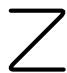
\includegraphics[keepaspectratio]{images/part002_abf04123.jpg}}

Remark. Note that the relation \(\mathbf{f} \sim \mathbf{g}\) by no means implies that the difference \(\mathbf{f} - \mathbf{g}\) tends to 0 along \(\mathfrak{F}\) ; this difference can even be unbounded, as is shown by the example \(x^{2} + x \sim x^{2}\) as \(x\) tends to \(+\infty\) .

PROPOSITION 8. Let K be a valued field and \(f_{1}, f_{2}, g_{1}, g_{2}\) four functions in \(\mathcal{H}(\mathfrak{F}, \mathrm{K})\) ; then the relations \(f_{1} \sim g_{1}\) and \(f_{2} \sim g_{2}\) imply \(f_{1}f_{2} \sim g_{1}g_{2}\) .

Indeed, we have \(f_{1}f_{2}-g_{1}g_{2}=f_{1}(f_{2}-g_{2})+(f_{1}-g_{1})g_{2}\) ; since \(f_{1}\preccurlyeq g_{1}\) , \(f_{1}-g_{1}\ll g_{1}\) and \(f_{2}-g_{2}\ll g_{2}\) , we have \(f_{1}f_{2}-g_{1}g_{2}\ll g_{1}g_{2}\) (V, p.~215, prop. 5 and 6).

In contrast, we have given an example in V, p.~214 where one has \(f_{1} = g_{1}\) , \(f_{2} \sim g_{2}\) and yet the relation \(f_{1} + f_{2} \asymp g_{1} + g_{2}\) does not hold (so neither a fortiori does

\[
f _ {1} + f _ {2} \sim g _ {1} + g _ {2}).
\]

The comparison relations \(f \ll g\) , \(f \sim g\) are called strong relations. Two functions f, g from \(\mathcal{H}(\mathfrak{F}, V)\) are called comparable (or strongly comparable when one wants to avoid any possible confusion) if they satisfy one of the three relations: \(f \ll g\) , \(f \gg g\) , or ``there exists a \(\lambda \neq 0\) such that \(f \sim g\lambda\) ''.

Remarks. 1) Two functions can be weakly comparable though not strongly comparable, for example the functions 1 and \(\sin x\) as \(x\) tends to \(+\infty\) .

\begin{enumerate}
\def\labelenumi{\arabic{enumi})}
\setcounter{enumi}{1}
\tightlist
\item
  In the definitions of the comparison relations \(f_{1} \preccurlyeq f_{2}\) and \(f_{1} \ll f_{2}\) the norms on the spaces \(V_{1}, V_{2}\) where \(f_{1}\) and \(f_{2}\) respectively take their values, are involved only apparently; in reality only the topologies on \(V_{1}\) and \(V_{2}\) are involved, for the relations \(f_{1} \preccurlyeq f_{2}\) and \(f_{1} \ll f_{2}\) are replaced by equivalent relations when one replaces the norm on \(V_{1}\) or \(V_{2}\) by an equivalent norm (Gen.~Top., IX, p.~170, def. 7).
\end{enumerate}

\subsection{CHANGE OF VARIABLE}

Let \(\varphi\) be a map from the set \(E'\) into \(E\) such that \(\overset{-1}{\varphi}(\mathfrak{F})\) is a filter base on \(E'\) . It is clear that if \(\mathbf{f}_1, \mathbf{f}_2\) are functions in \(\mathcal{H}(\mathfrak{F}, V_1)\) and \(\mathcal{H}(\mathfrak{F}, V_2)\) respectively, then \(\mathbf{f}_1 \circ \varphi\) , \(\mathbf{f}_2 \circ \varphi\) belong to \(\mathcal{H}(\overset{-1}{\varphi}(\mathfrak{F}), V_1)\) and \(\mathcal{H}(\overset{-1}{\varphi}(\mathfrak{F}), V_2)\) respectively, and that the relation \(\mathbf{f}_1 \preccurlyeq \mathbf{f}_2\) (resp. \(\mathbf{f}_1 \ll \mathbf{f}_2\) ) is equivalent to \(\mathbf{f}_1 \circ \varphi \preccurlyeq \mathbf{f}_2 \circ \varphi\) (resp. \(\mathbf{f}_1 \circ \varphi \ll \mathbf{f}_2 \circ \varphi\) ).

\subsection{COMPARISON RELATIONS BETWEEN STRICTLY POSITIVE FUNCTIONS}

Let \(g\) be a function in \(\mathcal{H}(\mathfrak{F},\mathbf{R})\) which is strictly positive on a set in \(\mathfrak{F}\) . Comparison relations featuring \(g\) can be formulated in another way: the relation \(\mathbf{f} \preccurlyeq g\) is equivalent to saying that \(\| \mathbf{f}\| /g\) (which is defined on a set in \(\mathfrak{F}\) ) is bounded on a set in \(\mathfrak{F}\) ; the relation \(\mathbf{f} \ll g\) is equivalent to saying that \(\| \mathbf{f}\| /g\) tends to 0 along \(\mathfrak{F}\) . If \(f\) is a function in \(\mathcal{H}(\mathfrak{F},\mathbf{R})\) the relation \(f\asymp g\) means that \(f / g\) is logarithmically bounded on a set in \(\mathfrak{F}\) , and the relation \(f\sim g\) that \(f / g\) tends to 1 along \(\mathfrak{F}\) . If \(f\) is a function in \(\mathcal{H}(\mathfrak{F},\mathbf{R})\) and positive on a set in \(\mathfrak{F}\) , to say that \(f\) and \(g\) are comparable implies that \(f / g\) tends to a limit (finite or equal to \(+\infty\) ) along \(\mathfrak{F}\) .

PROPOSITION 9. Let \(f\) and \(g\) be two functions in \(\mathcal{H}(\mathfrak{F},\mathbf{R})\) , strictly positive on a set in \(\mathfrak{F}\) . For \(f\) and \(g\) to be comparable it is necessary and sufficient that for every number \(t \geqslant 0\) , with at most one exception, the function \(f - tg\) has constant sign \(^3\) on a set in \(\mathfrak{F}\) .

The condition is necessary. Indeed, if \(f \ll g\) one has \(f - tg \sim -tg\) except for \(t = 0\) , so \(f - tg\) is strictly negative on a set in \(\mathfrak{F}\) , except for \(t = 0\) ; if \(f \gg g\) then \(f - tg\) is strictly positive on a set in \(\mathfrak{F}\) for all \(t\) ; finally, if \(f \sim kg\) ( \(k\) constant \(> 0\) ), then \(f - tg \sim (k - t)g\) except for \(t = k\) , so, except perhaps for \(t = k\) , \(f - tg\) has the sign of \(k - t\) on a set in \(\mathfrak{F}\) .

The condition is sufficient. Indeed, suppose that the ratio \(f / g\) has two distinct cluster points \(\alpha < \beta\) along \(\mathfrak{F}\) . For every number \(t\) such that \(\alpha < t < \beta\) there then exist in every set \(X \in \mathfrak{F}\) two points \(x_{1}, x_{2}\) such that \(f(x_{1}) / g(x_{1}) < t\) and \(f(x_{2}) / g(x_{2}) > t\) ; thus \(f(x) - tg(x)\) does not have constant sign on \(X\) ; we have arrived at a conclusion incompatible with the hypothesis. It follows that \(f / g\) can have only one cluster value (finite or infinite) along the filter with base \(\mathfrak{F}\) , and consequently, (Gen.~Top., I, p.~85, corollary) has this value as its limit along \(\mathfrak{F}\) .

PROPOSITION 10. Let \(f\) and \(g\) be two functions in \(\mathcal{H}(\mathfrak{F},\mathbf{R})\) which are strictly positive on a set in \(\mathfrak{F}\) ; for every \(\alpha\) real and \(\neq 0\) the relation \(f\asymp g\) (resp. \(f\sim g\) ) is equivalent to \(f^{\alpha}\asymp g^{\alpha}\) (resp. \(f^{\alpha}\sim g^{\alpha}\) ); if \(\alpha >0\) the relation \(f\preccurlyeq g\) (resp. \(f\ll g\) ) is equivalent to \(f^{\alpha}\preccurlyeq g^{\alpha}\) (resp. \(f^{\alpha}\ll g^{\alpha}\) ); if \(\alpha < 0\) it is equivalent to \(f^{\alpha}\succcurlyeq g^{\alpha}\) (resp. \(f^{\alpha}\gg g^{\alpha}\) ).

The proofs are immediate.

One notes that in \(\mathcal{H}(\mathfrak{F},\mathbf{R})\) the set \(\varGamma\) of functions strictly positive on a set in F is such that \(\varGamma/\mathrm{R}_{\infty}\) is a multiplicative group \(\varGamma_{\infty}\) in \(\mathcal{H}_{\infty}(\mathfrak{F},\mathbf{R})\) ; \(\varGamma/\mathrm{R}_{0}\) is identical to the quotient group of \(\varGamma_{\infty}\) by the subgroup of classes (mod. \(R_{\infty}\) ) of logarithmically bounded functions in \(\varGamma\) ; on \(\varGamma/R_{0}\) the order relation deduced from the relation \(f \preccurlyeq g\) by passage to the quotient is compatible with the group structure of \(\varGamma/R_{0}\) and thus makes it an ordered group.

PROPOSITION 11. Let g be a function in \(\mathcal{H}(\mathfrak{F},\mathbf{R})\) such that \(\lim_{\mathfrak{F}}g = +\infty\) ; the relation \(f \ll g\) implies \(e^{f} \ll e^{g}\) ; the relation \(f \sim g\) implies \(\log f \sim \log g\) .

Indeed, if \(f \ll g\) then \(f - g = g\left(\frac{f}{g} - 1\right)\) tends to \(-\infty\) along \(\mathfrak{F}\) . Similarly, if \(f \sim g\) one has \(\log f = \log g + \log \frac{f}{g}\) , so \(\log f - \log g\) tends to 0, and the same for \(\frac{\log f}{\log g} - 1 = \frac{\log f - \log g}{\log g}\) .

\pandocbounded{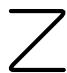
\includegraphics[keepaspectratio]{images/part002_2162bedd.jpg}}

On the other hand, note that the relation \(f \sim g\) does not imply \(e^{f} \sim e^{g}\) , nor even that \(e^{f} \asymp e^{g}\) , as is shown by the example where \(f(x) = x^{2}\) , \(g(x) = x^{2} + x\) as x tends to \(+\infty\) ; similarly, the relation \(f \ll g\) does not imply \(\log f \ll \log g\) , as is shown by the example \(f(x) = x\) , \(g(x) = x^{2}\) as x tends to \(+\infty\) .

DEFINITION 5. Let g be a function in \(\mathcal{H}(\mathfrak{F},\mathbf{R})\) , strictly positive on a set in F, and such that \(\lim_{\mathfrak{F}}g=0\) or \(\lim_{\mathfrak{F}}g=+\infty\) . One says that a function \(f\in\mathcal{H}(\mathfrak{F},\mathbf{R})\) is of order \(\rho\) (finite or infinite) relative to g if \(\lim_{\mathfrak{F}}\log(|f|)/\log g=\rho\) .

Note that if f is of order \(\rho\) relative to g then f is of order \(-\rho\) relative to 1/g; one therefore need treat only the case where \(g(x)\) tends to \(+\infty\) along F.

\pandocbounded{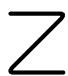
\includegraphics[keepaspectratio]{images/part002_5139c9a2.jpg}}

PROPOSITION 12. Let \(g\) be a function in \(\mathcal{H}(\mathfrak{F},\mathbf{R})\) such that \(\lim_{\mathfrak{F}}g = +\infty\) ; let \(f\) be a function in \(\mathcal{H}(\mathfrak{F},\mathbf{R})\) .

\begin{enumerate}
\def\labelenumi{\alph{enumi})}
\item
  For \(f\) to be of order \(+\infty\) relative to \(g\) it is necessary and sufficient that \(f \gg g^{\alpha}\) for every \(\alpha \geqslant 0\) .
\item
  For \(f\) to be of order \(-\infty\) relative to \(g\) it is necessary and sufficient that \(f \ll g^{-\alpha}\) for every \(\alpha > 0\) .
\item
  For \(f\) to be of finite order equal to \(\rho\) relative to \(g\) it is necessary and sufficient that, for every \(\varepsilon > 0\) , one has \(g^{\rho - \varepsilon} \ll f \ll g^{\rho + \varepsilon}\) .
\end{enumerate}

Let us prove c) for example. If the order of \(f\) relative to \(g\) is \(\rho\) then for every \(\varepsilon > 0\) there exists a set \(\mathbf{M} \in \mathfrak{F}\) such that, for every \(x \in \mathbf{M}\) , we have

\[
\left(\rho - \frac {\varepsilon}{2}\right) \log g (x) \leqslant \log | f (x) | \leqslant \left(\rho + \frac {\varepsilon}{2}\right) \log g (x),
\]

or \((g(x))^{\rho-\frac{\varepsilon}{2}} \leqslant |f(x)| \leqslant (g(x))^{\rho+\frac{\varepsilon}{2}}\) ; since \(\lim_{\mathfrak{F}} g = +\infty\) one thus has \(g^{\rho-\varepsilon} \ll f \ll g^{\rho+\varepsilon}\) for every \(\varepsilon > 0\) ; the converse is immediate. The proofs of a) and b) are similar.

Note that if \(f\) is of finite order \(\rho\) relative to \(g\) then \(fg^{-\rho}\) is of order 0 relative to \(g\) , and conversely; if \(f_1\) (resp. \(f_2\) ) is of order \(\rho_1\) (resp. \(\rho_2\) ) relative to \(g\) , and if \(\rho_1 + \rho_2\) is defined, then \(f_1f_2\) is of order \(\rho_1 + \rho_2\) relative to \(g\) .

Remarks. 1) Observe that though f may be of finite order \(\rho\) relative to g nevertheless the ratio \(f/g^{\rho}\) need not tend to a limit; for example, every logarithmically bounded function is of order 0 relative to g, but need not have a limit along F.

\begin{enumerate}
\def\labelenumi{\arabic{enumi})}
\setcounter{enumi}{1}
\tightlist
\item
  A function defined on a set in \(\mathfrak{F}\) need not have a determinate order (finite or not) relative to \(g\) , for the functions having a determinate order relative to \(g\) are comparable to all the powers of \(g\) with at most one exception. Now \(f\) need not have this property, as one sees from the example \(g(x) = x\) , \(f(x) = 1 + x^2 \sin^2 x\) (as \(x\) tends to \(+\infty\) ). In this example \(f\) is comparable to \(g^\alpha\) for \(\alpha < 0\) and \(\alpha > 2\) ; if one takes \(f(x) = e^x \sin^2 x + e^{-x} \cos^2 x\) then \(f\) is not comparable to any power (positive or negative) of \(g\) .
\end{enumerate}

\subsection{NOTATION}

Given a real function \(f \in \mathcal{H}(\mathfrak{F}, \mathbf{R})\) it is often convenient in a formula to write \(O(f)\) for a function dominated by \(f\) , and \(o(f)\) for a negligible function relative to \(f\) . When, in a proof, there feature several functions dominated by the same function \(f\) (resp. negligible relative to \(f\) ) we denote them by \(O_1(f)\) , \(O_2(f)\) , etc. (resp. \(o_1(f)\) , \(o_2(f)\) , etc.).

Many authors write \(O(f)\) (resp. \(o(f)\) ) indiscriminately for all functions in a proof that are dominated by f (resp. negligible relative to f), an abuse of language which may risk confusion.

With this notation we can express props. 1, 2, 3 (V, p.~213) as follows: if \(g = O_1(f)\) and \(h = O(g)\) then \(h = O_2(f)\) ; one can write

\[
\sum_ {i = 1} ^ {n} \lambda_ {i} O _ {i} (f) = O _ {n + 1} (f) \quad (\lambda_ {i} \text {   scalars })\tag{1}
\]

\[
O (f) O (g) = O (f g).\tag{2}
\]

Similarly, prop. 4 (V, p.~215) shows that if \(g = O_1(f)\) and \(h = o(g)\) (resp. \(g = o_1(f)\) and \(h = O(g)\) then \(h = o_2(f)\) , and props. 5 and 6 (V, p.~5) can be expressed in the form

\[
\sum_ {i = 1} ^ {n} \lambda_ {i} o _ {i} (f) = o _ {n + 1} (f) \quad (\lambda_ {i} \text {   scalars })\tag{3}
\]

\[
o (f) O (g) = o (f g).\tag{4}
\]

The relation \(f \sim g\) is equivalent to \(f = g + o(g)\) . The notation \(O(1)\) (resp. \(o(1)\) ) denotes a function bounded on a set in \(\mathfrak{F}\) (resp. a function tending to 0 along \(\mathfrak{F}\) ).

\section{ASYMPTOTIC EXPANSIONS}

\subsection{SCALES OF COMPARISON}

Let E be a set filtered by a filter with base F, and K a non-discrete valued field (most often K = R or K = C). In the set of functions in \(\mathcal{H}(\mathfrak{F}, \mathrm{K})\) not equivalent to 0 modulo \(R_{\infty}\) (that is, those for which in every set in F there is at least one point where the function does not vanish), the relation `` \(f \ll g\) or f = g'' is an order relation.

DEFINITION 1. One says that a subset E of \(\mathcal{H}(\mathfrak{F},\mathrm{K})\) formed of functions not equivalent to 0 modulo \(R_{\infty}\) is a comparison scale when E is totally ordered by the relation `` \(f \ll g\) or f = g''.

In other words, if \(f\) and \(g\) are functions in \(\mathcal{E}\) then one (and only one) of the relations \(f \ll g\) , \(g \ll f\) , \(f = g\) always holds. It follows that on \(\mathcal{E}\) the relation \(f \asymp g\) (and a fortiori \(|f| \sim a |g|\) , where \(a\) is a number \(> 0\) ) implies \(f = g\) .

Every subset of a comparison scale is clearly also a comparison scale.

Examples. 1) For x real and tending to \(+\infty\) the set of functions \(x^{\alpha}\) ( \(\alpha\) an arbitrary real number) is a comparison scale. The same is true for the functions \((x - a)^{\alpha}\) when F is the set of open intervals with left-hand endpoint a.

\begin{enumerate}
\def\labelenumi{\arabic{enumi})}
\setcounter{enumi}{1}
\item
  For \(z\) complex tending to \(\infty\) the set of functions \(z^n\) ( \(n\) a rational integer) is a comparison scale; so are the functions \((z - a)^n\) when \(\mathfrak{F}\) is the trace on the complement of the point \(a \in \mathbf{C}\) of the filter of neighbourhoods of this point.
\item
  Let F be normed space; the family of functions \(\|\mathbf{x}-\mathbf{a}\|^{\alpha}\) ( \(\alpha\) an arbitrary real number) is a comparison scale when F is the trace on the complement of a of the filter of neighbourhoods of this point. Note that if p and q are two distinct norms on F, the union of the two comparison scales \(\left(p(\mathbf{x}-\mathbf{a})\right)^{\alpha}\) and \(\left(q(\mathbf{x}-\mathbf{a})\right)^{\alpha}\) is not in general a comparison scale.
\item
  For \(x\) real tending to \(+\infty\) the family \(\mathcal{E}\) of functions of the form \(\exp(p(x))\) , where \(p\) runs through the set of polynomials without constant term (with real coefficients), is a comparison scale: it suffices to remark that the quotient of two functions in \(\mathcal{E}\) is again in \(\mathcal{E}\) , and that a function \(\exp(p(x))\) must tend either to 0 or \(+\infty\) if \(p \neq 0\) ; indeed, \(p(x) \sim \alpha x^n\) where \(n > 0\) and \(\alpha \neq 0\) ; if \(\alpha > 0\) then \(p(x) > \frac{1}{2}\alpha x^n\) for \(x\) sufficiently large; if \(\alpha < 0\) then \(p(x) < \frac{1}{2}\alpha x^n\) for \(x\) sufficiently large; in the first case \(\exp(p(x))\) tends to \(+\infty\) , in the second to 0.
\item
  For x real tending to \(+\infty\) the set E of functions of the form \(x^{\alpha}(\log x)^{\beta}\) (defined for x \textgreater{} 1), where \(\alpha\) and \(\beta\) are arbitrary real numbers, is a comparison scale. Indeed, here again the quotient of two functions in E is a function in E; it is enough to show that if \(\alpha\) and \(\beta\) are not both zero then \(x^{\alpha}(\log x)^{\beta}\) tends to 0 or \(+\infty\) ; this is clear if \(\alpha = 0, \beta \neq 0\) ; if \(\alpha > 0\) one has \((\log x)^{-\beta} \ll x^{\alpha}\) , and if \(\alpha < 0\) one has \((\log x)^{\beta} \ll x^{-\alpha}\) for any \(\beta\) , whence the proposition.
\end{enumerate}

Note that this last comparison scale is a totally ordered set (for the relation `` \(f \ll g\) or \(f = g\) '') whose order structure is isomorphic to the lexicographic order on \(R^{2}\) (Set Theory, III, p.~157); recall that in this structure the relation \((\alpha, \beta) < (\gamma, \delta)\) means `` \(\alpha < \gamma\) , or \(\alpha = \gamma\) and \(\beta < \delta\) '').

Similarly, the scale formed by the functions \(\exp(p(x))\) , where p runs through the set \(P_{0}\) of polynomials with no constant term, has order structure isomorphic to the order structure of \(P_{0}\) , in which the relation p \textless{} q implies that the dominant term of the polynomial q - p has a coefficient \textgreater{} 0 (cf.~Alg., VI. 19, Example 2).

Let \(\varphi\) be a map from a set \(F\) into \(E\) , such that \(\overset{-1}{\varphi}(\mathfrak{F})\) is a filter base on \(F\) . If \(\mathcal{E}\) is a comparison scale on \(E\) (for the filter base \(\mathfrak{F}\) ) then the functions \(f \circ \varphi\) , as \(f\) runs through \(\mathcal{E}\) , form a comparison scale on \(F\) (for the filter base \(\overset{-1}{\varphi}(\mathfrak{F})\) ).

\subsection{PRINCIPAL PARTS AND ASYMPTOTIC EXPANSIONS}

Let E be a comparison scale formed by functions with values in a non-discrete valued field K. Let V be a normed space over K, and let f be a function in \(\mathcal{H}(\mathfrak{F}, V)\) ; if there are a function \(g \in E\) and an element \(a \neq 0\) in V such that \(f \sim ag\) , one says that ag is a principal part of f relative to the scale E. From def. 1 of V, p.~10, f can have only one principal part relative to E, for if \(g_{1}\) , \(g_{2}\) are two functions in E and \(a_{1}\) , \(a_{2}\) are two \(\neq 0\) elements of V, then the relation \(a_{1}g_{1} \sim a_{2}g_{2}\) implies \(|g_{1}| \asymp |g_{2}|\) and consequently \(g_{1} = g_{2}\) , whence \((\mathbf{a}_{2} - \mathbf{a}_{1})g_{1} \ll g_{1}\) , and since \(g_{1}\) is not identically zero on any set in E this implies \(a_{2} = a_{1}\) .

If f has a principal part relative to a comparison scale E it has the same principal part relative to every comparison scale \(E' \supset E\) .

Examples. 1) For x real (resp. complex) tending to \(+\infty\) (resp. \(\infty\) ), every polynomial \(a_{0}x^{n} + a_{1}x^{n-1} + \ldots + a_{n}\) with coefficients in V, such that \(a_{0} \neq 0\) , has principal part \(a_{0}x^{n}\) with respect to the scale \(x^{n}\) (or any scale containing the \(x^{n}\) ). It follows that every rational fraction \(\frac{a_{0}x^{n} + \cdots + a_{m}}{b_{0}x^{n} + \cdots + b_{n}}\) with real or complex coefficients such that \(a_{0}b_{0} \neq 0\) has principal part \(\frac{a_{0}}{b_{0}}x^{m-n}\) with respect to the same scale.

\begin{enumerate}
\def\labelenumi{\arabic{enumi})}
\setcounter{enumi}{1}
\tightlist
\item
  A function may be comparable to all the functions of a scale and yet not admit a principal part with respect to this scale. For example, for \(x\) real tending to \(+\infty\) , \(\sqrt{x}\) has no principal part with respect to the scale \(x^n\) where \(n\) is a rational integer; \(\log x\) has no principal part with respect to the scale of \(x^\alpha\) ( \(\alpha\) arbitrary real); \(\exp(\sqrt{\log x})\) and \(x^x = e^{x\log x}\) have no principal part with respect to the scale of the \(x^\alpha (\log x)^\beta\) , nor with respect to the scale of the \(\exp(p(x))\) ( \(p\) a polynomial with no constant term).
\end{enumerate}

The concept of principal part admits extensive generalization. Suppose that a function \(\mathbf{f} \in \mathcal{H}(\mathfrak{F}, V)\) has a principal part \(\mathbf{a}_1g_1\) with respect to a scale \(\mathcal{E}\) ; the relation \(\mathbf{f} \sim \mathbf{a}_1g_1\) is equivalent to \(\mathbf{f} - \mathbf{a}_1g_1 \ll g_1\) (V, p.~216, def. 4); to study the function \(\mathbf{f}\) more closely one is thus led to consider the function \(\mathbf{f} - \mathbf{a}_1g_1\) . If this function has a principal part \(\mathbf{a}_2g_2\) with respect to \(\mathcal{E}\) one must have \(g_2 \ll g_1\) and \(\mathbf{f} - \mathbf{a}_1g_1 - \mathbf{a}_2g_2 \ll g_2\) .

More generally, suppose that the scale E is written parametrically in the form \((g_{\alpha})\) where \(\alpha\) runs through a set of indices A endowed with a totally ordered structure isomorphic to the opposite of the order structure of E: the relation \(\alpha < \beta\) is thus equivalent to \(g_{\beta} \ll g_{\alpha}\) . In these circumstances:

DEFINITION 2. One says that a function \(\mathbf{f} \in \mathcal{H}(\mathfrak{F}, V)\) admits an asymptotic expansion to precision \(g_{\alpha}\) (relative to the scale \(\mathcal{E}\) ) if there exists a family \((\mathbf{a}_{\lambda})_{\lambda \leqslant \alpha}\) of elements of V, all but a finite number of them being 0, such that \(\mathbf{f} - \sum_{\lambda \leqslant \alpha} \mathbf{a}_{\lambda} g_{\lambda} \ll g_{\alpha}\) . One says that \(\sum_{\lambda \leqslant \alpha} \mathbf{a}_{\lambda} g_{\lambda}\) is an asymptotic expansion of \(\mathbf{f}\) to precision \(g_{\alpha}\) , that the \(\mathbf{a}_{\lambda} g_{\lambda} (\lambda \leqslant \alpha)\) are its terms, the \(\mathbf{a}_{\lambda}\) its coefficients, and the function \(\mathbf{r}_{\alpha} = \mathbf{f} - \sum_{\lambda \leqslant \alpha} \mathbf{a}_{\lambda} g_{\lambda}\) the remainder of this expansion.

To express the fact that \(\sum_{\lambda \leqslant \alpha} \mathbf{a}_{\lambda} g_{\lambda}\) is an asymptotic expansion of \(\mathbf{f}\) to precision \(g_{\alpha}\) one most often restricts oneself to writing

\[
\mathbf {f} = \sum_ {\lambda \leqslant \alpha} \mathbf {a} _ {\lambda} g _ {\lambda} + o (g _ {\alpha}) \quad (\text { or } \mathbf {f} = \sum_ {\lambda \leqslant \alpha} \mathbf {a} _ {\lambda} g _ {\lambda} + o _ {k} (g _ {\alpha})
\]

if there are several functions in the proof) following the notation of V, p.~219 and 220.

Of two asymptotic expansions (of two functions, distinct or not) relative to the same scale E, one says that the one with precision of greater index is the more precise.

If \(\sum_{\lambda \leqslant \alpha} \mathbf{a}_{\lambda} g_{\lambda}\) is an asymptotic expansion of \(\mathbf{f}\) to precision \(g_{\alpha}\) , then, for every \(\beta < \alpha\) , \(\sum_{\lambda \leqslant \beta} \mathbf{a}_{\lambda} g_{\lambda}\) is an asymptotic expansion of \(\mathbf{f}\) to precision \(g_{\beta}\) (V, p.~215, prop. 5): one says that it is obtained by reducing the precision of the given expansion \(\sum_{\lambda \leqslant \alpha} \mathbf{a}_{\lambda} g_{\lambda}\) of \(\mathbf{f}\) to \(g_{\beta}\) .

If \(\sum_{\lambda \leqslant \alpha} \mathbf{a}_{\lambda} g_{\lambda}\) and \(\sum_{\lambda \leqslant \alpha} \mathbf{b}_{\lambda} g_{\lambda}\) are asymptotic expansions to the same precision \(g_{\alpha}\) of two functions \(\mathbf{f}_1, \mathbf{f}_2\) , then \(\sum_{\lambda \leqslant \alpha} (\mathbf{a}_{\lambda} + \mathbf{b}_{\lambda}) g_{\lambda}\) is an asymptotic expansion of \(\mathbf{f}_1 + \mathbf{f}_2\) to

precision \(g_{\alpha}\) (V, p.~215, prop. 5); and for every scalar \(c\) , \(\sum_{\lambda \leqslant \alpha} \mathbf{a}_{\lambda}cg_{\lambda}\) is an asymptotic expansion of \(\mathbf{f}_1c\) to precision \(g_{\alpha}\) . It follows that if a function admits an asymptotic expansion to precision \(g_{\alpha}\) then this expansion is unique: it is sufficient to see that the function 0 does not admit an asymptotic expansion with precision \(g_{\alpha}\) having coefficients \(\neq 0\) . For, if \(0 = \sum_{\lambda \leqslant \alpha} \mathbf{a}_{\lambda}g_{\lambda} + \mathbf{r}_{\alpha}\) , and if \(\gamma\) were the least of the indices \(\lambda \leqslant \alpha\) such that \(\mathbf{a}_{\lambda} \neq 0\) , one would have \(\mathbf{a}_{\gamma}g_{\gamma} = -\sum_{\gamma < \lambda \leqslant \alpha} \mathbf{a}_{\lambda}g_{\lambda} - \mathbf{r}_{\alpha} \ll g_{\gamma}\) , which is absurd.

To say that a function \(\mathbf{f}\) admits an asymptotic expansion to precision \(g_{\alpha}\) , all of whose coefficients are zero, is equivalent to saying that \(\mathbf{f} \ll g_{\alpha}\) . If \(\mathbf{f}\) admits an asymptotic expansion \(\sum_{\lambda \leqslant \alpha} \mathbf{a}_{\lambda} g_{\lambda}\) to precision \(g_{\alpha}\) whose coefficients are not all zero, and if \(\gamma\) is the smallest of the indices \(\lambda\) such that \(\mathbf{a}_{\lambda} \neq 0\) , then \(\mathbf{a}_{\gamma} g_{\gamma}\) is the principal part of \(\mathbf{f}\) relative to the scale \(\mathcal{E}\) , for one has \(\mathbf{f} - \mathbf{a}_{\gamma} g_{\gamma} = \sum_{\gamma < \lambda \leqslant \alpha} \mathbf{a}_{\lambda} g_{\lambda} + \mathbf{r}_{\alpha} \ll g_{\gamma}\) ; similarly, if \(\mu \leqslant \alpha\) is an index such that \(\mathbf{a}_{\mu} \neq 0\) , then \(\mathbf{a}_{\mu} g_{\mu}\) is the principal part of \(\mathbf{f} - \sum_{\lambda < \mu} \mathbf{a}_{\lambda} g_{\lambda}\) .

The most important asymptotic expansions in applications are those relative to the scale of the \(x^{-n}\) (resp. of the \(z^{-n}\) ), where n is a positive or negative integer, as x tends to \(+\infty\) or to \(-\infty\) (resp. when the complex number z tends to \(\infty\) ), or relative to the scale of the \((x - c)^{n}\) (resp. \((z - c)^{n}\) ) when the real number x tends to c from the right or left (resp. when the complex number z tends to c). We saw in I, p.~21 that every vector function of a real variable x which is k times differentiable at a point \(c \in R\) admits a Taylor expansion of order k at this point, that is, an asymptotic expansion to precision \((x - c)^{k}\) with respect to the scale of the \((x - c)^{n}\) .

\subsection{SUMS AND PRODUCTS OF ASYMPTOTIC EXPANSIONS}

If \(f_{1}\) , \(f_{2}\) admit asymptotic expansions to precision \(g_{\alpha}\) and \(g_{\beta}\) respectively, relative to a comparison scale E, one deduces expansions to precision \(g_{\min(\alpha,\beta)}\) by limiting the two expansions to this precision; we have seen in V, p.~222 how one obtains an asymptotic expansion for \(f_{1} + f_{2}\) to precision \(g_{\min(\alpha,\beta)}\) .

Let \(V_{1}, V_{2}\) and V be three normed spaces over the field K, and let \((\mathbf{x}, \mathbf{y}) \mapsto [\mathbf{x}, \mathbf{y}]\) be a continuous bilinear map from \(V_{1} \times V_{2}\) into V; we suppose further, for the rest of this section, that the scale E is such that the product of any two functions in E is again in E (which is true for all the comparison scales given as examples (in V, p.~220)).

Now let \(f_{1}\) , \(f_{2}\) be two functions in \(\mathcal{H}(\mathfrak{F}, V_{1})\) and \(\mathcal{H}(\mathfrak{F}, V_{2})\) respectively, having asymptotic expansions \(f_{1} = \sum_{\lambda \leqslant \alpha} a_{\lambda} g_{\lambda} + r_{\alpha}\) and \(f_{2} = \sum_{\mu \leqslant \beta} b_{\mu} g_{\mu} + r_{\beta}\) to precision \(g_{\alpha}\) and \(g_{\beta}\) respectively, with respect to the scale E. Suppose further that neither the \(a_{\lambda}\) nor the \(b_{\mu}\) are all zero, and let \(a_{\gamma} g_{\gamma}\) and \(b_{\delta} g_{\delta}\) be the principal parts of \(f_{1}\) and \(f_{2}\) . By hypothesis, one can write \(g_{\gamma} g_{\beta} = g_{\rho}\) and \(g_{\delta} g_{\alpha} = g_{\sigma}\) ; let us show that the sum \(\sum[a_{\lambda}.b_{\mu}]g_{\lambda}g_{\mu}\) taken over all pairs \((\lambda,\mu)\) such that \(g_{\min(\rho,\sigma)}\ll g_{\lambda}g_{\mu}\) , is an asymptotic expansion of \([f_{1}.f_{2}]\) to precision \(g_{\min(\rho,\sigma)}\) . Now the difference between \([f_{1}.f_{2}]\) and this sum is the sum of a finite number of terms, each of which is either of the form \([a_{\lambda}.b_{\mu}]g_{\lambda}g_{\mu}\) with \(g_{\lambda}g_{\mu}\ll g_{\min(\rho,\sigma)}\) , or of the form \([a_{\lambda}.r_{\beta}]g_{\lambda}\) where \(\lambda\geqslant\gamma\) , or of the form \([r_{\alpha}.b_{\mu}]g_{\mu}\) where \(\mu\geqslant\delta\) ; but since {[}x.y{]} is continuous, one has from (V, p.~213, prop. 3 and V, p.~215, prop. 6) that \([a_{\lambda}.r_{\beta}]g_{\lambda}\preccurlyeq r_{\beta}g_{\lambda}\ll g_{\beta}g_{\gamma}=g_{\rho}\) for \(\lambda\geqslant\gamma\) , and similarly \([r_{\alpha}.b_{\mu}]g_{\mu}\preccurlyeq r_{\alpha}g_{\mu}\ll g_{\alpha}g_{\delta}=g_{\sigma}\) for \(\mu\geqslant\delta\) , whence the proposition (V, p.~215, prop. 5).

If all the \(a_{\lambda}\) are zero one has \([f_{1}.f_{2}] \ll g_{\alpha}g_{\delta}\) ; in other words, one has an asymptotic expansion of \([f_{1}.f_{2}]\) with zero terms, to precision \(g_{\alpha}g_{\delta}\) ; similarly if all the \(a_{\lambda}\) and \(b_{\mu}\) are zero one has an asymptotic expansion of \([f_{1}.f_{2}]\) with zero terms to precision \(g_{\alpha}g_{\beta}\) .

We shall apply the preceding result principally to the case where V is a normed algebra over K and the bilinear function \([x.y]\) is the product xy in this algebra; the most important cases are those where V is equal to R or to C.

In particular, if \(f_{i}\) ( \(1 \leqslant i \leqslant n\) ) are n functions in \(\mathcal{H}(\mathfrak{F}, \mathrm{K})\) each of which admits an asymptotic expansion with respect to E one can obtain an asymptotic expansion with respect to E for every polynomial \(\sum_{(v_{i})} a_{v_{1}v_{2}\ldots v_{n}} f_{1}^{v_{1}} \ldots f_{n}^{v_{n}}\) in the \(f_{i}\) with coefficients in a normed space V; furthermore, the preceding rules allow one to determine the precision of the expansion obtained, if one knows those of the expansions of the functions \(f_{i}\) .

\subsection{COMPOSITION OF ASYMPTOTIC EXPANSIONS}

Let f be a function in \(\mathcal{H}(\mathfrak{F},\mathbf{R})\) (resp. \(\mathcal{H}(\mathfrak{F},\mathbf{C})\) ), admitting an asymptotic expansion to precision \(g_{\alpha}\) with respect to a scale E, and having limit 0 along the filter with base F. On the other hand let h be a function with values in a normed space V over R (resp. C), defined on a neighbourhood of the point 0 in R (resp. C), and n times differentiable on this neighbourhood; then

\[
\mathbf {h} (t) = \mathbf {c} _ {0} + \mathbf {c} _ {1} t + \dots + \mathbf {c} _ {n} t ^ {n} + o (t ^ {n})
\]

on this neighbourhood (I, p.~21), whence, on a suitable set in \(\mathfrak{F}\)

\[
\mathbf {h} \circ f = \mathbf {c} _ {0} + \mathbf {c} _ {1} f + \dots + \mathbf {c} _ {n} f ^ {n} + o (f ^ {n}).
\]

We have seen, in n° 3, how to form an asymptotic expansion for \(c_{0} + c_{1}f + \cdots + c_{n}f^{n}\) to a precision \(g_{\rho}\) determined by the precision of the expansion of f; moreover, suppose that the coefficients of the asymptotic expansion of f are not all zero, and that \(a_{\gamma}g_{\gamma}\) is the principal part of f, and let \(g_{\sigma} = g_{\gamma}^{n}\) ; if \(\sigma < \rho\) one will have an expansion of \(h \circ f\) to precision \(g_{\sigma}\) on limiting the expansion of \(\sum_{k=0}^{n} c_{k}f^{k}\) to this precision; if, on the contrary, \(\rho \leqslant \sigma\) , then the expansion of \(\sum_{k=0}^{n} c_{k}f^{k}\) is also an expansion of \(h \circ f\) to precision \(g_{\rho}\) .

If all the terms of the asymptotic expansion of \(f\) are zero, and if \(g_{\alpha} \ll 1\) , then \(f \ll g_{\alpha}\) and so \(f^k \ll g_{\alpha}^k \ll g_{\alpha}\) for every integer \(k > 0\) ; if \(\mathbf{c}_m\) is the first coefficient of index \(> 0\) which is not zero (assuming that the \(\mathbf{c}_k\) for indices \(k > 0\) are not all 0), then \(\mathbf{c}_0\) is an asymptotic expansion of \(\mathbf{h} \circ f\) to precision \(g_{\alpha}^{m}\) .

In the remainder of this section we shall restrict ourselves to the case where the functions in \(\mathcal{E}\) have real values and are strictly positive on a set in \(\mathfrak{F}\) , and we shall consider asymptotic expansions only of functions in \(\mathcal{H}(\mathfrak{F},\mathbf{R})\) . Suppose first that for every function \(g\in \mathcal{E}\) and every real number \(\nu\) , \(g^{\nu}\) again belongs to \(\mathcal{E}\) : this condition is fulfilled, for example, by the scale of the \(x^{\alpha}\) or by that of the \(x^{\alpha}|\log x|^{\beta}\) ( \(\alpha\) and \(\beta\) being arbitrary real numbers) on a neighbourhood of \(+\infty\) or a neighbourhood of 0 in \(\mathbf{R}\) . This property implies that the quotient of two functions in \(\mathcal{E}\) again belongs to \(\mathcal{E}\) . This being so, from an asymptotic expansion relative to \(\mathcal{E}\) of a function \(f\in \mathcal{H}(\mathfrak{F},\mathbf{R})\) , to precision \(g_{\alpha}\) , one can derive an expansion for \(|f|^{\nu}\) for every real number \(\nu\) . Let us restrict ourselves to the case where the coefficients of the expansion of \(f\) are not all zero, and let \(a_{\gamma}g_{\gamma}\) be the principal part of \(f\) ; one can write \(|f|^{\nu} = |a_{\gamma}|^{\nu}g_{\gamma}^{\nu}(1 + h)^{\nu}\) , with

\[
h = \sum_ {\gamma <   \lambda \leqslant \alpha} \frac {a _ {\lambda}}{a _ {\gamma}} \frac {g _ {\lambda}}{g _ {\gamma}} + o \left(\frac {g _ {\alpha}}{g _ {\gamma}}\right).
\]

Under our hypotheses \(\sum_{\gamma < \lambda \leqslant \alpha} \frac{a_{\lambda}}{a_{\gamma}} \frac{g_{\lambda}}{g_{\gamma}}\) is an asymptotic expansion of \(h\) , to precision \(g_{\alpha} / g_{\gamma}\) ; since \(h\) tends to 0 along \(\mathfrak{F}\) the method described above gives an asymptotic expansion of \((1 + h)^{\nu}\) , then an expansion of \(|f|^{\nu}\) on multiplying by \(\left|a_{\gamma}\right|^{\nu} g_{\gamma}^{\nu}\) .

With the same hypotheses on \(f\) one can write

\[
\log | f | = \log \left| a _ {\gamma} g _ {\gamma} \right| + \log (1 + h)
\]

and \(\log(1+h)\) can be expanded, as has been said above, the function \(\log(1+t)\) being indefinitely differentiable on a neighbourhood of 0; if, further, \(\log g_{\gamma}\) admits an asymptotic expansion with respect to E, or with respect to a scale \(E_{1} \supset E\) , one obtains an asymptotic expansion for \(\log|f|\) on adding the two asymptotic expansions.

Example. We have \((1+x)^{1/x}=\exp\left(\frac{1}{x}\log(1+x)\right)\) ; when x tends to \(+\infty\) we have \(\log(1+x)=\log x+\log\left(1+\frac{1}{x}\right)\) , whence the asymptotic expansion of \(\frac{1}{x}\log(1+x)\) with respect to the scale of the \(x^{\alpha}(\log x)^{\beta}\) :

\[
\frac {1}{x} \log (1 + x) = \frac {\log x}{x} + \frac {1}{x ^ {2}} - \frac {1}{2 x ^ {3}} + o _ {1} \left(\frac {1}{x ^ {3}}\right).
\]

From this expansion, and from the Taylor expansion

\[
e ^ {u} = 1 + u + \frac {u ^ {2}}{2} + \frac {u ^ {3}}{6} + o (u ^ {3})
\]

on a neighbourhood of u = 0, one deduces the asymptotic expansion

\[
\begin{array}{r l} (1 + x) ^ {1 / x} & = 1 + \frac {\log x}{x} + \frac {1}{2} \frac {(\log x) ^ {2}}{x ^ {2}} + \frac {1}{x ^ {2}} \\ & \quad + \frac {1}{6} \frac {(\log x) ^ {3}}{x ^ {3}} + \frac {\log x}{x ^ {3}} - \frac {1}{2 x ^ {3}} + o _ {2} \left(\frac {1}{x ^ {3}}\right) \end{array}
\]

with respect to the scale \(x^{\alpha}(\log x)^{\beta}\) by the methods explained above.

Keeping the same hypotheses and notation, the asymptotic expansion of \(e^{f}\) does not pose new problems except when \(f \gg 1\) ; one must then distinguish two cases, as \(g_{\alpha} \gg 1\) or \(g_{\alpha} \preccurlyeq 1\) . In the first case, giving an expansion for f does not allow one to obtain a principal part for \(e^{f}\) relative to E, because one does not know in general whether the remainder \(r_{\alpha}\) tends to 0, that is, whether \(e^{r_{\alpha}}\) tends to 1. On the contrary, if \(g_{\alpha} \preccurlyeq 1\) then \(r_{\alpha} \ll 1\) and so \(e^{f} \sim \exp\left(\sum_{\lambda \leqslant \alpha} a_{\lambda} g_{\lambda}\right)\) . One can make this result more precise: let \(a_{\gamma} g_{\gamma}\) be the principal part of f and let \(\delta\) be the index (such that \(\gamma < \delta \leqslant \alpha\) ) for which \(g_{\delta} = 1\) ; we put \(f_{1} = \sum_{\lambda \leqslant \delta} a_{\lambda} g_{\lambda}\) , \(f_{2} = \sum_{\delta < \lambda \leqslant \alpha} a_{\lambda} g_{\lambda} + r_{\alpha}\) ; we have \(f = f_{1} + f_{2}\) , so \(e^{f} = e^{f_{1}} e^{f_{2}}\) , and the general method explained at the start of this subsection allows one to form an asymptotic expansion of \(e^{f_{2}}\) (starting from the Taylor expansion of \(e^{t}\) at the point t = 0). One will then have an asymptotic expansion for \(e^{f}\) if \(e^{f_{1}} = \prod_{\lambda \leqslant \delta} \exp(a_{\lambda} g_{\lambda})\) belongs to E, or to a scale \(E_{1}\) containing E.

Example. We have \(x^{x^{1/x}} = \exp\left(\log x. \exp\left(\frac{1}{x} \log x\right)\right)\) ; when x tends to \(+\infty\) one has \(\log x \ll x\) , whence the asymptotic expansion of \(\log x. \exp\left(\frac{1}{x} \log x\right)\) with respect to the scale \(x^{\alpha}(\log x)^{\beta}\) :

\[
\log x. \exp \left(\frac {1}{x} \log x\right) = \log x + \frac {(\log x) ^ {2}}{x} + \frac {1}{2} \frac {(\log x) ^ {3}}{x ^ {2}} + o \left(\frac {(\log x) ^ {3}}{x ^ {2}}\right).
\]

All the terms of this expansion, starting from the second, tend to 0; from this expansion and from the Taylor expansion \(e^u = 1 + u + u^2 / 2 + o(u^2)\) on a neighbourhood of \(u = 0\) one deduces

\[
x ^ {x ^ {1 / x}} = x + (\log x) ^ {2} + \frac {1}{2} \frac {(\log x) ^ {4}}{x} + \frac {1}{2} \frac {(\log x) ^ {3}}{x} + o \left(\frac {(\log x) ^ {3}}{x}\right).
\]

\subsection{ASYMPTOTIC EXPANSIONS WITH VARIABLE COEFFICIENTS}

One can generalize the concept of principal part, and that of an asymptotic expansion, in the following way. Let E be a comparison scale formed of real (resp. complex) functions such that, for each of them, there is a set in F on which the function does not vanish at any point. Further, let C be a set of functions in \(\mathcal{H}(\mathfrak{F}, V)\) satisfying the following three conditions:

\((\mathrm{CO}_{\mathrm{I}})\) For every function \(\mathbf{a} \in \mathcal{C}\) one has \(\mathbf{a} \preccurlyeq 1\) .

\((\mathrm{CO}_{\mathrm{II}})\) The relation \(\mathbf{a} \ll 1\) for a function \(\mathbf{a} \in \mathcal{C}\) implies \(\mathbf{a} = 0\) .

\((\mathrm{CO}_{\mathrm{III}})\mathcal{C}\) is a vector space over R (resp. C).

Now let \(\mathbf{f}\) be any function in \(\mathcal{H}(\mathfrak{F}, V)\) ; if there exist a function \(g \in \mathcal{E}\) and a nonzero function \(\mathbf{a} \in \mathcal{C}\) such that \(\mathbf{f} - \mathbf{a}g \ll g\) one will say that \(\mathbf{a}g\) is a principal part of \(\mathbf{f}\) , relative to the comparison scale \(\mathcal{E}\) and to the domain of coefficients \(\mathcal{C}\) . If such a principal part exists, it is unique: for suppose that there are two principal parts \(\mathbf{a}_1g_1\) and \(\mathbf{a}_2g_2\) ; one cannot have \(g_1 \ll g_2\) since from \((\mathrm{CO_I})\) one could deduce that \(\mathbf{a}_1g_1 \ll g_2\) and \(\mathbf{f} - \mathbf{a}_1g_1 \ll g_1 \ll g_2\) , so \(\mathbf{f} \ll g_2\) ; but one would also have \(\mathbf{a}_2g_2 \ll g_2\) and consequently \(\mathbf{a}_2 \ll 1\) contradicting the hypothesis \(\mathbf{a}_2 \neq 0\) and \((\mathrm{CO_{II}})\) . So one must have \(g_1 = g_2\) ; from the relations \(\mathbf{f} - \mathbf{a}_1g_1 \ll g_1, \mathbf{f} - \mathbf{a}_2g_1 \ll g_1\) one deduces that \((\mathbf{a}_2 - \mathbf{a}_1)g_1 \ll g_1\) whence \(\mathbf{a}_2 - \mathbf{a}_1 \ll 1\) , and consequently \(\mathbf{a}_2 = \mathbf{a}_1\) , by \((\mathrm{CO_{II}})\) and \((\mathrm{CO_{III}})\) .

Example. For \(x\) real tending to \(+\infty\) the periodic bounded functions on \(\mathbf{R}\) , having the same period \(\tau\) , satisfy conditions \((\mathrm{CO}_{\mathrm{I}})\) , \((\mathrm{CO}_{\mathrm{II}})\) and \((\mathrm{CO}_{\mathrm{III}})\) : if \(\lim_{x\to +\infty}a(x) = 0\) then for every \(\varepsilon >0\) there is an \(x_0\) such that \(|a(x)|\leqslant \varepsilon\) for every \(x\geqslant x_0\) ; one deduces that \(|a(x)|\leqslant \varepsilon\) for \(0\leqslant x\leqslant \tau\) too, since there exists an integer \(n\) such that \(x + n\tau \geqslant x_0\) , and such that \(a(x) = a(x + n\tau)\) ; since \(\varepsilon\) is arbitrary one has \(a(x) = 0\) on \([0,\tau]\) , hence everywhere.

With the notation of V, p.~222, we will say that \(\sum_{\lambda \leqslant \alpha} \mathbf{a}_{\lambda} g_{\lambda}\) , where the \(\mathbf{a}_{\lambda}\) belong to \(\mathcal{C}\) and all but a finite number of them are zero, is an asymptotic expansion of \(\mathbf{f}\) with coefficients in \(\mathcal{C}\) , to precision \(g_{\alpha}\) , if \(\mathbf{f} - \sum_{\lambda \leqslant \alpha} \mathbf{a}_{\lambda} g_{\lambda} \ll g_{\alpha}\) ; for every index \(\mu\) such that \(\mathbf{a}_{\mu} \neq 0\) then \(\mathbf{a}_{\mu} g_{\mu}\) is the principal part of \(\mathbf{f} - \sum_{\lambda < \mu} \mathbf{a}_{\lambda} g_{\lambda}\) , relative to \(\mathcal{E}\) and to \(\mathcal{C}\) , which proves the uniqueness of the asymptotic expansion of \(\mathbf{f}\) (to precision \(g_{\alpha}\) ) when it exists.

The methods given in \(n^{\circ}\) 3 (V, p.~223) for forming an asymptotic expansion for \(f_{1} + f_{2}\) or for \([f_{1}.f_{2}]\) , starting from given asymptotic expansions for \(f_{1}\) and \(f_{2}\) , can again be applied to expansions with variable coefficients, so long as the \([a_{\lambda}.b_{\mu}]\) belong to the domain of coefficients C corresponding to the normed space V or admit an asymptotic expansion with coefficients in C.

\section{ASYMPTOTIC EXPANSIONS OF FUNCTIONS OF A REAL VARIABLE}

In this section we shall consider only the case where the set E is an open interval in the extended real line \(\overline{R}\) , and F is a base for the trace on E of the filter of neighbourhoods of the left or right-hand endpoint \(\alpha\) of E; further, we shall study above all the (finite) real functions defined on a set in F (depending on the function under consideration).

Using one of the changes of variable \(x' = -x\) , \(x' = \frac{1}{x - \alpha}\) , \(x' = -\frac{1}{x - \alpha}\) as needed, one can always reduce to the case where E is an interval of the form \(]a, +\infty[\) so that F will be formed of intervals \([t, +\infty[\) with t \textgreater{} a. We shall restrict ourselves principally to this latter case, and leave the task of translating most of the propositions we obtain (by the above changes of variable) to the reader, except for a few particularly important results.

It will be convenient to employ an abuse of language and refer to the sets in \(\mathfrak{F}\) as ``neighbourhoods of \(+\infty\)''.

\subsection{INTEGRATION OF COMPARISON RELATIONS: I. WEAK RELATIONS}

PROPOSITION 1. Let \(\mathbf{f}\) be a regulated vector function, \(g\) a regulated function \(\geqslant 0\) on an interval \([a, +\infty[\) , such that \(\int_{a}^{+\infty} g(t) dt > 0\) . The relation \(\mathbf{f} \preccurlyeq g\) as \(x\) tends to \(+\infty\) implies that \(\int_{a}^{x} \mathbf{f}(t) dt \preccurlyeq \int_{a}^{x} g(t) dt\) . If the integral \(\int_{a}^{+\infty} g(t) dt\) converges then the integral \(\int_{a}^{+\infty} \mathbf{f}(t) dt\) converges absolutely.

Indeed, by hypothesis there exist a \(b \geqslant a\) and a number \(c' > 0\) such that

\[
\| \mathbf {f} (x) \| \leqslant c ^ {\prime} g (x) \quad \text {   for   } x \geqslant b,
\]

whence

\[
\left\| \int_ {b} ^ {x} \mathbf {f} (t) d t \right\| \leqslant \int_ {b} ^ {x} \| \mathbf {f} (t) \| d t \leqslant c ^ {\prime} \int_ {b} ^ {x} g (t) d t;
\]

since, moreover, one may suppose \(b\) so large that \(\int_{a}^{b} g(t) dt > 0\) , there exists a \(c'' > 0\) such that \(\left\| \int_{a}^{b} \mathbf{f}(t) dt \right\| \leqslant c'' \int_{a}^{b} g(t) dt\) ; on putting \(c = \max(c', c'')\) one thus has

\[
\left\| \int_ {a} ^ {x} \mathbf {f} (t) d t \right\| \leqslant c \int_ {a} ^ {x} g (t) d t
\]

for every \(x \geqslant b\) , whence the proposition.

COROLLARY 1. If \(f\) and \(g\) are regulated functions and \(\geqslant 0\) on the interval \([a, +\infty[\) , and such that \(f \succcurlyeq g\) , and if \(\int_{a}^{+\infty} g(t) dt = +\infty\) , then \(\int_{a}^{+\infty} f(t) dt = +\infty\) .

COROLLARY 2. If \(f\) and \(g\) are \(\geqslant 0\) and not identically zero on \([a, +\infty[\) , and such that \(f \asymp g\) , then \(\int_{a}^{x} f(t) dt \asymp \int_{a}^{x} g(t) dt\) .

\subsection{APPLICATION: LOGARITHMIC CRITERIA FOR CONVERGENCE OF INTEGRALS}

By choosing the function g suitably one can deduce criteria for deciding whether the integral \(\int_{a}^{+\infty} f(t) dt\) of a function \(f \geqslant 0\) converges or is infinite from prop. 1 of V, p.~228, and cor. 1 thereto: it suffices to choose for g a function whose primitive is known. In particular, since \(x^{\mu}\) has primitive \(\frac{x^{\mu+1}}{\mu+1}\) when \(\mu \neq -1\) , and \(\log x\) when \(\mu = -1\) , we have the following criterion:

PROPOSITION 2 (``logarithmic criterion of order 0''). Let f be a regulated function \(\geqslant 0\) on an interval \([a, +\infty[\); if \(f(x) \preccurlyeq x^{\mu}\) for some \(\mu < -1\) then the integral \(\int_{a}^{+\infty} f(t) dt\) converges; if \(f(x) \succcurlyeq x^{\mu}\) for some \(\mu \geqslant -1\) then the integral \(\int_{a}^{+\infty} f(t) dt\) is infinite.

This criterion is not decisive when \(1 / x^{1 + \alpha} \ll f(x) \ll 1 / x\) for every exponent \(\alpha > 0\) , as, for example, when \(f(x) = 1 / x(\log x)^{\mu}\) ( \(\mu > 0\) ). But in this last case \(f\) has primitive \(\frac{1}{1 - \mu} (\log x)^{1 - \mu}\) if \(\mu \neq 1\) and \(\log \log x\) when \(\mu = 1\) . Thus:

PROPOSITION 3 (``logarithmic criterion of order 1''). Let f be a regulated function \(\geqslant 0\) on an interval \([a, +\infty[\); if \(f(x) \preccurlyeq 1/x(\log x)^{\mu}\) for some \(\mu > 1\) then the integral \(\int_{a}^{+\infty} f(t) dt\) converges; if \(f(x) \succcurlyeq 1/x(\log x)^{\mu}\) for some \(\mu \leqslant 1\) then the integral \(\int_{a}^{+\infty} f(t) dt\) is infinite.

Generally, for every integer \(n \geqslant 0\) , let us denote by \(l_{n}(x)\) the function defined inductively (for x large enough) by the relations \(l_{0}(x) = x\) , \(l_{n}(x) = \log(l_{n-1}(x))\) for \(n \geqslant 1\) ; one says that \(l_{n}(x)\) is the \(n^{th}\) iterated logarithm of x (cf.~Appendix). One verifies immediately that \(\frac{1}{1 - \mu}\left(l_{n}(x)\right)^{1 - \mu}\) is a primitive of

\[
\frac {1}{x l _ {1} (x) l _ {2} (x) \dots l _ {n - 1} (x) \left(l _ {n} (x)\right) ^ {\mu}}
\]

for \(\mu \neq 1\) , and \(l_{n+1}(x)\) is a primitive of \(\frac{1}{xl_1(x)l_2(x)\ldots l_{n-1}(x)l_n(x)}\) . Hence:

PROPOSITION 4 (``logarithmic criterion of order n''). Let f be a regulated function \(\geqslant0\) on an interval \([a,+\infty[\); if, for some \(\mu>1\), \(f(x)\preccurlyeq\frac{1}{xl_{1}(x)l_{2}(x)\ldots l_{n-1}(x)(l_{n}(x))^{\mu}}\) , then the integral \(\int_{a}^{+\infty}f(t)dt\) converges; if \(f(x)\succcurlyeq\frac{1}{xl_{1}(x)l_{2}(x)\ldots l_{n-1}(x)(l_{n}(x))^{\mu}}\) for some \(\mu\leqslant1\) , then the integral \(\int_{a}^{+\infty}f(t)dt\) is infinite.

Each logarithmic criterion is thus applicable to functions for which the criteria of lower order are not decisive (cf.~V, p.~264, exerc. 5 b) and V, p.~265, exerc. 8).

Because of its usefulness we translate the criterion of order 0 for integrals \(\int_{\alpha}^{a}f(t)dt\) where \(f\) is regulated and \(\geqslant 0\) on a non-compact interval \([\alpha ,a]\) :

PROPOSITION 5 (``logarithmic criterion of order 0''). If on a neighbourhood of \(\alpha\) one has \(f(x) \preccurlyeq 1/(x - \alpha)^{\mu}\) for some \(\mu < 1\) then the integral \(\int_{\alpha}^{a} f(t) dt\) converges; if \(f(x) \succcurlyeq 1/(x - \alpha)^{\mu}\) for some \(\mu \geqslant 1\) then the integral \(\int_{\alpha}^{a} f(t) dt\) is infinite.

We leave it to the reader to translate the logarithmic criterion of order \(n\) similarly.

The application of the logarithmic criteria is immediate if one knows how to obtain the principal part of f with respect to a comparison scale containing the functions that feature in these criteria: if \(f_{1}\) is the principal part, the integral \(\int_{\alpha}^{+\infty} f(t) dt\) converges or is infinite together with \(\int_{\alpha}^{+\infty} f_{1}(t) dt\) , and the logarithmic criteria apply immediately to this last integral.

Examples. 1) The function \(t^p (1 - t)^q\) is not bounded on {]}0, 1{[} when \(p < 0\) or \(q < 0\) ; by the logarithmic criterion of order 0 applied on a neighbourhood of the points 0 and 1 the integral \(\int_0^1 t^p (1 - t)^q dt\) converges if and only if \(p > -1\) and \(q > -1\) . If so, this integral is called the Eulerian integral of the first kind and is denoted by \(\mathbf{B}(p + 1,q + 1)\) (cf.~VII, p.~312).

\begin{enumerate}
\def\labelenumi{\arabic{enumi})}
\setcounter{enumi}{1}
\tightlist
\item
  Consider the integral \(\int_0^\infty t^{x - 1}e^{-t}dt\) . Since \(e^{-t}\sim 1\) on a neighbourhood of 0, one must have \(x > 0\) if this integral is to converge; this condition is also sufficient since on a neighbourhood of \(+\infty\) one has \(e^{-t}\ll t^{-\mu}\) for any \(\mu >0\) . When \(x > 0\) the integral is called the Eulerian integral of the second kind and is denoted by \(\Gamma (x)\) (cf.~VII, p.~311).
\end{enumerate}

\subsection{INTEGRATION OF COMPARISON RELATIONS: II. STRONG RELATIONS}

PROPOSITION 6. Let \(\mathbf{f}\) be a regulated vector function, and \(g\) a regulated function \(\geqslant 0\) on \([a, +\infty[\) .

\(1^{\circ}\) If the integral \(\int_{a}^{+\infty} g(t) dt\) converges then the relation \(\mathbf{f} \ll g\) (resp. \(\mathbf{f} \sim \mathbf{c}g\) , where \(\mathbf{c}\) is constant) implies that \(\int_{x}^{+\infty} \mathbf{f}(t) dt \ll \int_{x}^{+\infty} g(t) dt\) (resp. \(\int_{x}^{+\infty} \mathbf{f}(t) dt \sim \mathbf{c} \int_{x}^{+\infty} g(t) dt\) ).

\(2^{\circ}\) If the integral \(\int_{a}^{+\infty} g(t) dt\) is infinite then the relation \(\mathbf{f} \ll g\) (resp. \(\mathbf{f} \sim \mathbf{c}g\) ) implies that

\[
\int_ {\alpha} ^ {x} \mathbf {f} (t) d t \ll \int_ {\beta} ^ {x} g (t) d t \quad (\text { resp. } \quad \int_ {\alpha} ^ {x} \mathbf {f} (t) d t \sim \mathbf {c} \int_ {\beta} ^ {x} g (t) d t),
\]

for any \(\alpha\) and \(\beta\) in \([a, +\infty[\) .

It is enough to prove the proposition for the relation \(\mathbf{f} \ll g\) since, if \(\mathbf{c} \neq 0\) , the relation \(\mathbf{f} \sim \mathbf{c}g\) is equivalent to \(\mathbf{f} - \mathbf{c}g \ll g\) .

The first part is an immediate consequence of the mean value theorem, since if \(\|\mathbf{f}(x)\| \leqslant \varepsilon g(x)\) for \(x \geqslant x_{0}\) one deduces that

\[
\left\| \int_ {x} ^ {+ \infty} \mathbf {f} (t) d t \right\| \leqslant \int_ {x} ^ {+ \infty} \| \mathbf {f} (t) \| d t \leqslant \varepsilon \int_ {x} ^ {+ \infty} g (t) d t \quad \text { for } x \geqslant x _ {0}.
\]

In the second place, suppose that \(\int_{a}^{+\infty} g(t) dt = +\infty\) . If \(\| \mathbf{f}(x) \| \leqslant \varepsilon g(x)\) for \(x \geqslant x_0 \geqslant \max(\alpha, \beta)\) , one has

\[
\begin{array}{l} \int_ {\alpha} ^ {x} \| \mathbf {f} (t) \| d t = \int_ {\alpha} ^ {x _ {0}} \| \mathbf {f} (t) \| d t + \int_ {x _ {0}} ^ {x} \| \mathbf {f} (t) \| d t \\ \leqslant \int_ {\alpha} ^ {x _ {0}} \| \mathbf {f} (t) \| d t + \varepsilon \int_ {x _ {0}} ^ {x} g (t) d t \\ = \varepsilon \int_ {\beta} ^ {x} g (t) d t + \left(\int_ {\alpha} ^ {x _ {0}} \| \mathbf {f} (t) \| d t - \varepsilon \int_ {\beta} ^ {x _ {0}} g (t) d t\right). \end{array}
\]

Now there exists an \(x_{1} \geqslant x_{0}\) such that for every \(x \geqslant x_{1}\)

\[
\left| \int_ {\alpha} ^ {x _ {0}} \| \mathbf {f} (t) \| d t - \varepsilon \int_ {\beta} ^ {x _ {0}} g (t) d t \right| \leqslant \varepsilon \int_ {\beta} ^ {x} g (t) d t
\]

whence, for \(x \geqslant x_1\)

\[
\left\| \int_ {\alpha} ^ {x} \mathbf {f} (t) d t \right\| \leqslant \int_ {\alpha} ^ {x} \| \mathbf {f} (t) \| d t \leqslant 2 \varepsilon \int_ {\beta} ^ {x} g (t) d t
\]

which completes the proof, since \(\varepsilon > 0\) is arbitrary.

In other words, one can integrate the two terms of a strong relation \(\mathbf{f} \ll g\) , \(\mathbf{f} \sim \mathbf{a}g\) , when \(g\) is positive on an interval \([a, +\infty[\) , and the relation persists between the primitives of the two terms, provided one takes care to integrate from \(x\) to \(+\infty\) if \(\int_{a}^{+\infty} g(t) dt\) converges, and from \(\alpha\) to \(x\) (for any \(\alpha\) in \([a, +\infty[\) ) in the opposite case.

Note that props. 1 (V, p.~228) and 6 (V, p.~230) remain valid when \(\mathfrak{F}\) is a base for the trace filter of the intervals \([t, +\infty[\) (where \(t > a\) ) on the complement of a countable set (cf.~I, p.~15, th. 2).

Examples. 1) On applying prop. 6 of V, p.~230, to the relation \(1 / x \ll x^{\alpha - 1}\) where \(\alpha > 0\) , one again obtains the relation \(\log x \ll x^{\alpha}\) for every \(\alpha > 0\) , which is equivalent to the relation \(y^{1 / \alpha} \ll e^{y}\) proved in III, p.~105.

\begin{enumerate}
\def\labelenumi{\arabic{enumi})}
\setcounter{enumi}{1}
\tightlist
\item
  We have \(\left(\frac{e^x}{x}\right)' = \frac{e^x}{x}\left(1 - \frac{1}{x}\right) \sim e^x / x\) ; since \(e^x / x\) tends to \(+\infty\) with \(x\) , one deduces from prop. 6 of V, p.~230, that \(\int_{1}^{x} \frac{e^t}{t} dt \sim e^x / x\) .
\end{enumerate}

Remark. When \(g\) is not assumed to remain \(\geqslant 0\) on an interval \([a, +\infty[\) (or to remain \(\leqslant 0\) on such an interval), and \(\int_{a}^{+\infty} g(t) dt\) is not convergent, the relation \(f \sim g\) does not necessarily imply that \(\int_{a}^{x} f(t) dt \sim \int_{a}^{x} g(t) dt\) , as is shown by the example where \(g(x) = \sin x\) and \(f(x) = \left(1 + \frac{\sin x}{x}\right) \sin x\) ; here

\pandocbounded{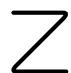
\includegraphics[keepaspectratio]{images/part002_ecaa53ed.jpg}}

\[
\int_ {n \pi} ^ {(n + 1) \pi} \frac {\sin^ {2} t}{t} d t \geqslant \frac {1}{(n + 1) \pi} \int_ {0} ^ {\pi} \sin^ {2} t d t \geqslant \frac {1}{2} \int_ {n + 1} ^ {n + 2} \frac {d t}{t},
\]

whence

\[
\int_ {\pi} ^ {n \pi} \frac {\sin^ {2} t}{t} d t \geqslant \frac {1}{2} \int_ {2} ^ {n + 1} \frac {d t}{t}
\]

and the integral \(\int_{1}^{+\infty} dt / t\) is infinite, though \(\int_{\frac{\pi}{2}}^{x} g(t) dt = -\cos x\) remains bounded (see V, p.~260, exerc. 4).

\subsection{DIFFERENTIATION OF COMPARISON RELATIONS}

\pandocbounded{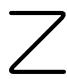
\includegraphics[keepaspectratio]{images/part002_390c97e1.jpg}}

Propositions 1 (V, p.~228) and 6 (V, p.~230) do not have converses: the existence of a comparison relation \(\mathbf{f} \preccurlyeq g\) , \(\mathbf{f} \ll g\) , \(\mathbf{f} \sim \mathbf{c}g\) between two functions that are differentiable on a neighbourhood of \(+\infty\) does not imply the same comparison relation between their derivatives, even for real monotone functions \(f\) and \(g\) .

For example, the function \(x^{2} + x\sin x + \cos x\) is monotone and equivalent to \(x^{2}\) , but its derivative \(x(2 + \cos x)\) is not equivalent to \(2x\) .

On the other hand, one can derive comparison relations when one assumes a priori that the derivatives of the functions considered are comparable (V, p.~217). In general, we shall say that two real functions f and g defined on an interval \([a, +\infty]\) are comparable to order k on a neighbourhood of \(+\infty\) if, on a neighbourhood of \(+\infty\) , they each have a regulated \(k^{th}\) derivative except at a countable set of points, and if, on this neighbourhood, \(f^{(k)}\) and \(g^{(k)}\) have constant sign (on the set on which they are defined) and are comparable.

We agree to say that two comparable real functions (V, p.~217) are comparable of order 0.

PROPOSITION 7. If two real functions \(f, g\) , are comparable of order 1, then they are comparable; further, the relation \(f \ll g\) (resp. \(f \sim cg\) , \(c\) constant) implies \(f' \ll g'\) (resp. \(f' \sim cg'\) ) unless \(g\) is equivalent to a nonzero constant.

Now, since \(f'\) and \(g'\) are of constant sign on an interval \([x_0, +\infty[\) , both \(f\) and \(g\) are monotone on this interval, so tend to a finite or infinite limit as \(x\) tends to \(+\infty\) . It is clear that \(f\) and \(g\) are comparable as \(x\) tends to \(+\infty\) if one of these limits is finite and \(\neq 0\) , or if one is zero and the other infinite. If both \(f\) and \(g\) tend to 0 one can write \(f(x) = -\int_x^{+\infty} f'(t) dt\) , \(g(x) = -\int_x^{+\infty} g'(t) dt\) ; since \(f'\) and \(g'\) are comparable the same is true for \(f\) and \(g\) and the comparison relation between \(f\) and \(g\) is the same as that between \(f'\) and \(g'\) , by prop. 6 (V, p.~20). Similarly, if \(f\) and \(g\) both have an infinite limit one has \(f(x) = f(x_0) + \int_{x_0}^x f'(t) dt\) , \(g(x) = g(x_0) + \int_{x_0}^x g'(t) dt\) ; again prop. 6 (V, p.~230) shows that \(f\) and \(g\) are comparable and that the comparison relation between \(f\) and \(g\) is the same as that between \(f'\) and \(g'\) . To complete the proof it remains to consider the case where \(g\) tends to \(\pm \infty\) and \(f\) to a constant; one cannot then have \(f' \succcurlyeq g'\) , since then one could deduce from prop. 1 (V, p.~218) that the integral \(\int_{x_0}^{+\infty} g'(t) dt\) was convergent; since \(f'\) and \(g'\) have been assumed comparable, one must have \(f' \ll g'\) .

COROLLARY. If two real functions \(f, g\) , are comparable of order \(k \geqslant 1\) , then they are comparable of order \(p\) for \(0 \leqslant p \leqslant k\) ; further, the relation \(f \ll g\) (resp. \(f \sim cg\) ) implies \(f^{(k)} \ll g^{(k)}\) (resp. \(f^{(k)} \sim cg^{(k)}\) ) unless one of the derivatives \(g^{(p)}\) ( \(0 \leqslant p \leqslant k - 1\) ) is equivalent to a constant \(\neq 0\) .

Indeed, since \(f^{(k)}\) and \(g^{(k)}\) have constant sign on an interval \([x_0, +\infty[\) , it follows that \(f^{(k-1)}\) and \(g^{(k-1)}\) are monotone on this interval, so have constant sign on a neighbourhood of \(+\infty\) ; further, prop. 7 of V, p.~232, shows that \(f^{(k-1)}\) and \(g^{(k-1)}\) are comparable, so the corollary follows from applying prop. 7 recursively.

Remarks. 1) The restriction on \(g\) in prop. 7 is essential. For example, one has \(\frac{1}{x} \ll 1 + \frac{1}{x}\) even though the derivatives of the two sides are equivalent; similarly \(1 + \frac{1}{x} \sim 1 + \frac{1}{x^2}\) , but \(1 / x^2 \gg 2 / x^3\) .

\begin{enumerate}
\def\labelenumi{\arabic{enumi})}
\setcounter{enumi}{1}
\item
  Though \(f\) and \(g\) are comparable of order \(k\) a function \(f_{1}\) equivalent to \(f\) need not be comparable of order \(k\) to \(g\) ; however it will be so if one assumes that \(f_{1}\) is comparable of order \(k\) to \(f\) and that none of the derivatives \(f^{(p)}\) ( \(0 \leqslant p \leqslant k - 1\) ) is equivalent to a nonzero constant.
\item
  If f and g are comparable of order k this need not be so for hf and hg even for a monotone function h as simple as \(h(x) = x\) (V, p.~260, exerc. 3); likewise, 1/f and 1/g are not necessarily comparable of order k (V, p.~259, exerc. 1).
\end{enumerate}

\subsection{PRINCIPAL PART OF A PRIMITIVE}

Let \(f\) be a regulated real function \(\neq 0\) having constant sign on an interval \([a, +\infty[\) ; the following proposition allows one to obtain the principal part of the primitive \(\int_{x}^{+\infty} f(t) dt\) if \(\int_{a}^{+\infty} f(t) dt\) converges in certain cases, and of the primitive \(\int_{a}^{x} f(t) dt\) if \(\int_{a}^{+\infty} f(t) dt\) is infinite:

PROPOSITION 8. Put \(\mathrm{F}(x) = \int_{x}^{+\infty} f(t) dt\) if \(\int_{a}^{+\infty} f(t) dt\) converges, and \(\mathrm{F}(x) = \int_{a}^{x} f(t) dt\) if \(\int_{a}^{+\infty} f(t) dt\) is infinite. Suppose that \(\log |f|\) and \(\log x\) are comparable of order 1.

\(1^{\circ}\) If \(f\) is of finite order \(\mu \neq -1\) with respect to \(x\) one has

\[
\mathrm{F} (x) \sim \frac {1}{| \mu + 1 |} x f (x).\tag{1}
\]

\(2^{\circ}\) If \(f\) is of infinite order relative to \(x\) and if \(f / f'\) and \(x\) are comparable of order 1, then one has

\[
\mathrm{F} (x) \sim \frac {(f (x)) ^ {2}}{| f ^ {\prime} (x) |}.\tag{2}
\]

One should note that the hypothesis implies that \(f(x)\) has a determinate order relative to \(x\) (V, p.~219).

\(1^{\circ}\) If \(f\) is of order \(\mu \neq 0\) relative to \(x\) one has \(\log |f| \sim \mu \log x\) , so, since \(\log |f|\) and \(\log x\) are comparable of order 1, by prop. 7 of V, p.~232 one has \(f'/f \sim\) \(\mu/x\) , whence \(xf' \sim \mu f\) . If \(\mu > -1\) one has \(f(x) \gg x^{\mu-\varepsilon}\) for every \(\varepsilon > 0\) , and hence (V, p.~229, prop. 2) the integral \(\int_{a}^{+\infty} f(t) dt\) is infinite. One can write \(F(x) = \int_{a}^{x} f(t) dt = xf(x) - af(a) - \int_{a}^{x} tf'(t) dt\) , whence again

\[
\int_ {a} ^ {x} \left(f (t) + t f ^ {\prime} (t)\right) d t = x f (x) - a f (a);
\]

since \(\mu \neq -1\) we have \(f(x) + xf'(x) \sim (\mu + 1)f(x)\) , so (V, p.~230, prop. 6)

\[
\int_ {a} ^ {x} \left(f (t) + t f ^ {\prime} (t)\right) d t \sim (\mu + 1) \mathrm{F} (x),
\]

which proves (1) in this case. If \(\mu = 0\) one has likewise that \(xf'(x) \ll f(x)\) , which again gives \(f(x) + xf'(x) \sim f(x)\) . One argues similarly when \(\mu < -1\) , in the case where \(\int_{a}^{+\infty} f(t) dt\) converges.

\(2^{\circ}\) If \(f\) is of order \(+\infty\) relative to \(x\) one has \(\log |f| \gg \log x\) , so (V, p.~232, prop. 7) \(f'/f \gg 1/x\) , or again, putting \(g(x) = f(x)/f'(x)\) , \(g(x) \ll x\) ; further, since \(f(x) \gg x^{\alpha}\) for every \(\alpha > 0\) the integral \(\int_{a}^{+\infty} f(t) dt\) is infinite. One can write

\[
\mathrm{F} (x) = \int_ {a} ^ {x} f (t) d t = \int_ {a} ^ {x} g (t) f ^ {\prime} (t) d t = g (x) f (x) - g (a) f (a) - \int_ {a} ^ {x} f (t) g ^ {\prime} (t) d t;
\]

since \(g\) and \(x\) are comparable of order 1, from the relation \(g(x) \ll x\) one can deduce (V, p.~232, prop. 7) that \(g'(x) \ll 1\) , hence that \(fg' \ll f\) , and consequently (V, p.~230, prop.6)

\[
\int_ {a} ^ {x} f (t) g ^ {\prime} (t) d t \ll \mathrm{F} (x),
\]

which establishes the relation (2). The proof is similar when \(f\) is of order \(-\infty\) relative to \(x\) , in the case where \(\int_{a}^{+\infty} f(t) dt\) converges.

Let E be a comparison scale (for real x tending to \(+\infty\) ) formed of nonzero real functions that are of constant sign on a neighbourhood of \(+\infty\) , such that \(x \in E\) and such that the product and quotient of two functions in E again belongs to E (V, p.~221 and p.~224). If a regulated function f with constant sign on a neighbourhood of \(+\infty\) has a principal part cg relative to E, then \(\int_{x}^{+\infty} f(t) dt\) (resp. \(\int_{a}^{x} f(t) dt\) according to the case) will be equivalent to \(c \int_{x}^{+\infty} g(t) dt\) (resp. \(c \int_{a}^{x} g(t) dt\) ); if the function g satisfies the hypotheses of prop. 8 of V, p.~233, and if (when the formula (2) of V, p.~233, applies) one knows a principal part of \(g'\) relative to E, one will thus have a principal part of \(\int_{x}^{+\infty} f(t) dt\) (resp. \(\int_{a}^{x} f(t) dt\) ) relative to E.

Examples. 1) The function \(1 / \log x\) is of order 0 relative to \(x\) and satisfies the conditions of prop. 8 of V, p.~233; thus

\[
\int_ {a} ^ {x} \frac {d t}{\log t} \sim \frac {x}{\log x}.
\]

\begin{enumerate}
\def\labelenumi{\arabic{enumi})}
\setcounter{enumi}{1}
\tightlist
\item
  The function \(e^{x^2}\) is of order \(+\infty\) relative to \(x\) and satisfies the conditions of prop. 8, so
\end{enumerate}

\[
\int_ {a} ^ {x} e ^ {t ^ {2}} d t \sim \frac {1}{2 x} e ^ {x ^ {2}}.
\]

In the Appendix (V, p.~252) we shall define a set of functions for which prop. 7 and prop. 8 always apply.

Remark. Prop. 8 does not apply directly to a function \(f\) of order \(-1\) relative to \(x\) . But then one can write \(f(x) = f_1(x) / x\) , with \(f_1\) of order 0 relative to \(x\) . Suppose, for example, that \(\int_{a}^{+\infty} f(t) dt\) is infinite; then

\[
\mathrm{F} (x) = \int_ {a} ^ {x} f (t) d t = \int_ {a} ^ {x} \frac {1}{t} f _ {1} (t) d t = \int_ {\log a} ^ {\log x} f _ {1} \left(e ^ {u}\right) d u.
\]

If the function \(f_{1}(e^{y})\) satisfies the hypotheses of prop. 8 and has an order \(\neq -1\) relative to \(y\) (that is, if \(f_{1}(x)\) has an order \(\neq -1\) relative to \(\log x\) ) the formulae (1) and (2) again allow us to obtain a principal part for \(F(x)\) . For example, let \(f(x) = \frac{\exp(\sqrt{\log x})}{x\log x}\) ; since \(\exp(\sqrt{\log x})\) is of order 0 relative to \(x\) , \(f\) is of order \(-1\) ; here one has \(f_{1}(e^{y}) = e^{\sqrt{y}} / y\) , and this function is of order \(+\infty\) relative to \(y\) ; prop. 8 applies and gives \(\int_{\alpha}^{y} e^{\sqrt{u}} / u du \sim 2e^{\sqrt{y}} / \sqrt{y}\) ; on reverting to the variable \(x\) we have \(\int_{a}^{x} \frac{\exp(\sqrt{\log t})}{t\log t} dt \sim \frac{2\exp(\sqrt{\log x})}{\sqrt{\log x}}\) .

\subsection{ASYMPTOTIC EXPANSION OF A PRIMITIVE}

Let E be a comparison scale on a neighbourhood of \(+\infty\) formed of real functions \(\neq 0\) of constant sign on a neighbourhood of \(+\infty\) ; let f be a regulated vector function defined on an interval \([a, +\infty[\) , with values in a complete normed space E, admitting an asymptotic expansion

\[
\mathbf {f} = \sum_ {\lambda \leqslant \alpha} \mathbf {a} _ {\lambda} g _ {\lambda} + \mathbf {r} _ {\alpha}
\]

to precision \(g_{\alpha}\) relative to E. Suppose further that every primitive \(\int_{a}^{x} g(t) dt\) of a function \(g \in E\) admits an asymptotic expansion with respect to E. In these circumstances we shall see that one can obtain an asymptotic expansion of \(\mathbf{F}(x) = \int_{a}^{x} \mathbf{f}(t) dt\) with respect to E. We distinguish two cases:

\(1^{\circ}\int_{a}^{+\infty}g_{\alpha}(t)dt\) is infinite; then one has \(\int_{a}^{x}\mathbf{r}_{\alpha}(t)dt\ll \int_{a}^{x}g_{\alpha}(t)dt\) (V,p.230, prop. 6); by hypothesis one can obtain an asymptotic expansion of \(\sum_{\lambda \leqslant \alpha}\mathbf{a}_{\lambda}\int_{a}^{x}g_{\lambda}(t)dt\)

to a certain precision \(g_{\rho}\) (V, p.~222); if \(cg_{\sigma}\) is the principal part of \(\int_{a}^{x} g_{\alpha}(t) dt\) one will thus have an asymptotic expansion of \(\int_{a}^{x} \mathbf{f}(t) dt\) to precision \(g_{\min(\rho, \sigma)}\) , with all the terms having indefinitely increasing norms.

\(2^{\circ}\int_{a}^{+\infty}g_{\alpha}(t)dt\) converges; let \(\beta\) then be the smallest of the indices \(\lambda \leqslant \alpha\) such that \(\mathbf{a}_{\lambda}\neq 0\) and such that \(\int_{a}^{+\infty}g_{\lambda}(t)dt\) converges; the integral

\[
\mathbf {C} = \int_ {a} ^ {+ \infty} \left(\mathbf {f} (t) - \sum_ {\lambda <   \beta} \mathbf {a} _ {\lambda} g _ {\lambda} (t)\right) d t
\]

is then convergent, and one can write

\[
\mathbf {F} (x) = \sum_ {\lambda <   \beta} \mathbf {a} _ {\lambda} \int_ {a} ^ {x} g _ {\lambda} (t) d t + \mathbf {C} - \sum_ {\beta \leqslant \lambda \leqslant \alpha} \mathbf {a} _ {\lambda} \int_ {x} ^ {+ \infty} g _ {\lambda} (t) d t - \int_ {x} ^ {+ \infty} \mathbf {r} _ {\alpha} (t) d t.
\]

Then \(\int_{x}^{+\infty}\mathbf{r}_{\alpha}(t)dt\ll \int_{x}^{+\infty}g_{\alpha}(t)dt\) ; if \(cg_{\sigma}\) is the principal part of \(\int_{x}^{+\infty}g_{\alpha}(t)dt\) , and if one has an asymptotic expansion of

\[
\sum_ {\lambda <   \beta} \mathbf {a} _ {\lambda} \int_ {a} ^ {x} g _ {\lambda} (t) d t + \mathbf {C} - \sum_ {\beta \leqslant \lambda \leqslant \alpha} \mathbf {a} _ {\lambda} \int_ {x} ^ {+ \infty} g _ {\lambda} (t) d t
\]

to precision \(g_{\rho}\) , one will as a result have an asymptotic expansion of \(\mathbf{F}\) to precision \(g_{\min(\rho, \sigma)}\) .

So it all amounts to finding asymptotic expansions with respect to E of primitives of functions in E. We have seen how, subject to certain hypotheses on E, prop. 8 of V, p.~233 gives the principal part of such a primitive. Further, the proof of prop. 8 gives the expression for the difference of the two sides of formula (1) (resp. (2)) of V, p.~233, in the form of a primitive of the function \(\frac{1}{|\mu+1|}\left(xf'(x)+f(x)\right)-f(x)\) (resp. \(f(x)g'(x)\) with \(g=f/f'\) ); on forming the principal part of this new primitive, as an asymptotic expansion of the right-hand side of (1) (resp. (2)), one obtains the right-hand side of the sought-for expansion (see V, p.~247-255).

Examples. 1) Let \(f(x) = 1 / \log x\) ( \(x > 1\) ); we have seen that \(\int_{a}^{x} dt / \log t \sim x / \log x\) , and that the difference \(\int_{a}^{x} \frac{dt}{\log t} - \frac{x}{\log x}\) is a primitive of \(1 / (\log x)^2\) ; one can apply prop. 8 again to this function, so obtaining \(\int_{a}^{x} dt / (\log t)^2 \sim x / (\log x)^2\) . By recursion one thus obtains the expansion

\[
\begin{array}{l} \int_ {a} ^ {x} \frac {d t}{\log t} = \frac {x}{\log x} + \frac {x}{(\log x) ^ {2}} \\ \qquad + \frac {2 x}{(\log x) ^ {3}} + \dots + (n - 1)! \frac {x}{(\log x) ^ {n}} + o \left(\frac {x}{(\log x) ^ {n}}\right). \end{array}
\]

Note that, irrespective of n, all the terms of this expansion tend to \(+\infty\) with x.

\begin{enumerate}
\def\labelenumi{\arabic{enumi})}
\setcounter{enumi}{1}
\tightlist
\item
  Let \(f(x) = \frac{e^x}{x^2 + 1}\) ; one can write \(f(x) = \frac{e^x}{x^2} - \frac{e^x}{x^4} + o_1\left(\frac{e^x}{x^4}\right)\) . Prop. 8 gives the expansions
\end{enumerate}

\[
\int_ {a} ^ {x} \frac {e ^ {t}}{t ^ {2}} d t = \frac {e ^ {x}}{x ^ {2}} + \frac {2 e ^ {x}}{x ^ {3}} + \frac {6 e ^ {x}}{x ^ {4}} + o _ {2} \left(\frac {e ^ {x}}{x ^ {4}}\right), \quad \int_ {a} ^ {x} \frac {e ^ {t}}{t ^ {4}} d t = \frac {e ^ {x}}{x ^ {4}} + o _ {3} \left(\frac {e ^ {x}}{x ^ {4}}\right)
\]

whence, on adding,

\[
\int_ {a} ^ {x} \frac {e ^ {t}}{t ^ {2} + 1} d t = \frac {e ^ {x}}{x ^ {2}} + 2 \frac {e ^ {x}}{x ^ {3}} + 5 \frac {e ^ {x}}{x ^ {4}} + o _ {4} \left(\frac {e ^ {x}}{x ^ {4}}\right).
\]

\section{APPLICATION TO SERIES WITH POSITIVE TERMS}
